\documentclass{beamer}
\graphicspath{ {graphics/}}
\usepackage[export]{adjustbox}

\begin{document}
\title{Literary Worlds Javascript Client}
\author{Tim Cunningham, John Lewis, Owen Watson}
\usenavigationsymbolstemplate{}
\frame{\titlepage}
\frame{\frametitle{Table of contents}\tableofcontents}

\section{Background}

\frame{\frametitle{Terms and Definitions}
\begin{itemize}
\item MUD (Multi User Domain)
  \begin{itemize}
    \item a networked, shared virtual environment
    \item provides a text based game for multiple users over the network
    \item Users move around rooms defined in the world
  \end{itemize}
\item MOO (MUD, Object Oriented)
  \begin{itemize}
    \item A MUD with objects that the user can interact with, create, and extend
  \end{itemize}
\item Client
  \begin{itemize}
    \item A program used to connect to a MUD server.
  \end{itemize}
\item Java applet
  \begin{itemize}
   \item A small application which is written in Java and can be executed in a web browser
  \end{itemize}
\item Telnet
  \begin{itemize}
    \item A network protocol used to provide an interactive text-oriented communication
  \end{itemize}
\end{itemize}
}

\frame{\frametitle{Background}
\begin{itemize}
  \item Literary Worlds is an MOO used for English education at many schools
  \item Many worlds have been created by students, teachers and professors based on various source material
  \item \textit{1984}, \textit{Brave New World}, \textit{Of Mice and Men}
\end{itemize}
}

\frame{\frametitle{Client}
\begin{itemize}
  \item Client: Allen Webb
  \item Professor of Comparative Literature and Postcolonial Studies at Western Michigan University's Department of English
  \item In 2003, Robert Rozema, a PhD student under Allen Webb created the prototype Literary World
  \item The Literary Worlds project was one of seven projects to receive funding from the Western Michigan University President's Innovation Fund
\end{itemize}
}

\frame{\frametitle{Goal of Project}
\begin{itemize}
  \item Existing interface is a Java applet
  \item Provide a new interface for Literary Worlds that works in modern browsers
  \begin{itemize}
    \item Google Chrome
    \item Firefox
    \item Internet Explorer
  \end{itemize}
  \item Use existing technology, unmodified

\end{itemize}
}

\frame{\frametitle{Literary Worlds}
  \begin{centering}
  \centerline{
  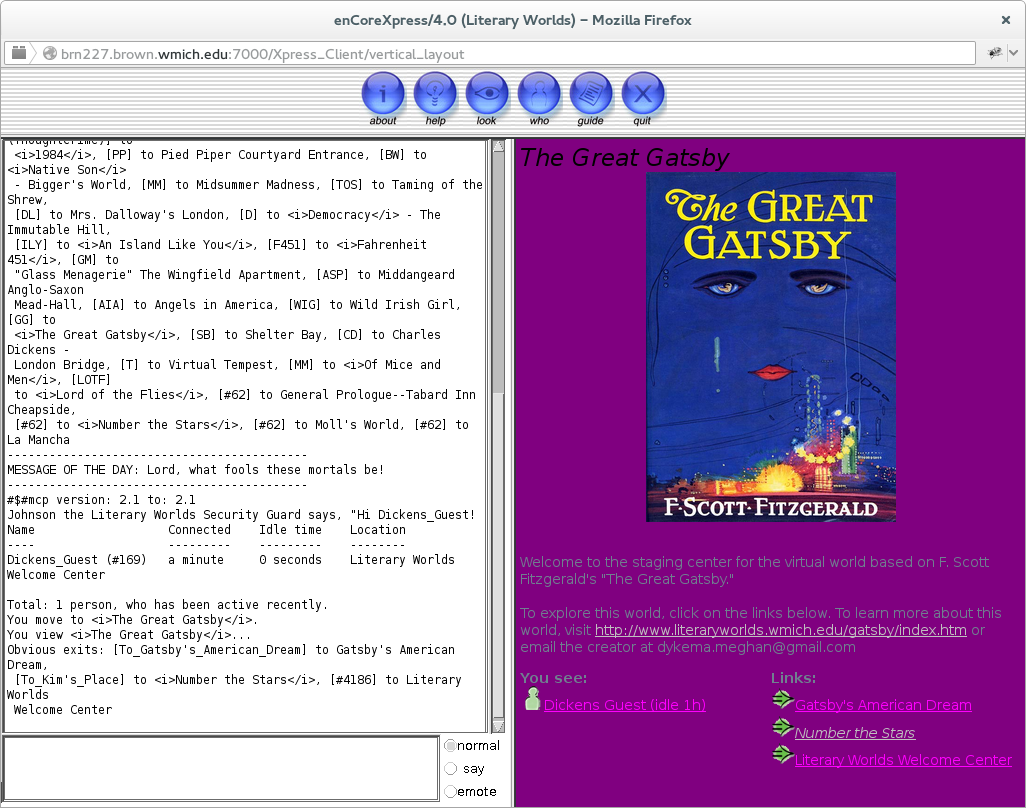
\includegraphics[width=0.75\textwidth,height=\textheight,keepaspectratio]{00_Great_Gatsby_Example.png}}
  \end{centering}
}

\frame{\frametitle{Literary Worlds}
  \begin{centering}
  \begin{itemize}
  \item Within these worlds, users can:
  \begin{itemize}
    \item Interact with characters
    % Both real and virtual (bots)
    \item Manipulate and interact with object
    % Examples given here
    \item Explore virtual environments
  \end{itemize}
  \end{itemize}
  \end{centering}
}

\frame{\frametitle{Example}
  \begin{centering}
  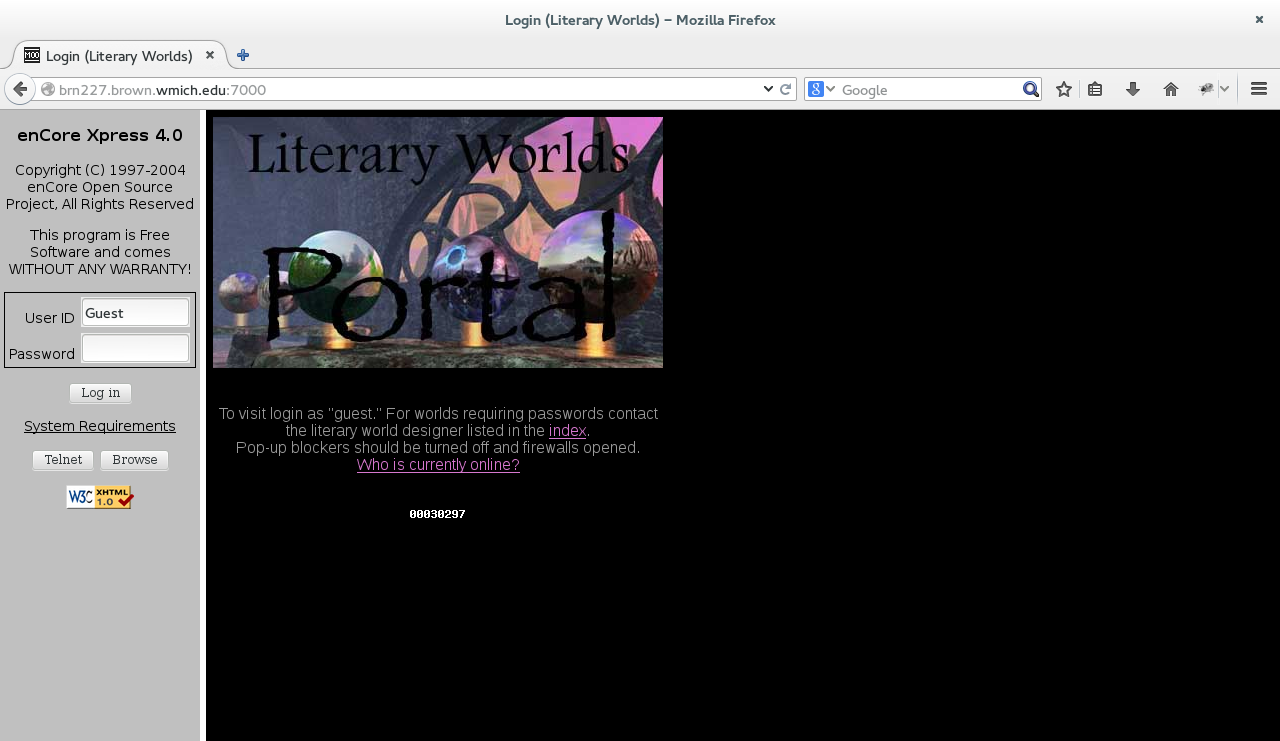
\includegraphics[width=\textwidth,height=\textheight,keepaspectratio]{01_LogIn.png}
  \end{centering}
}

\frame{\frametitle{Example}
  \begin{centering}
  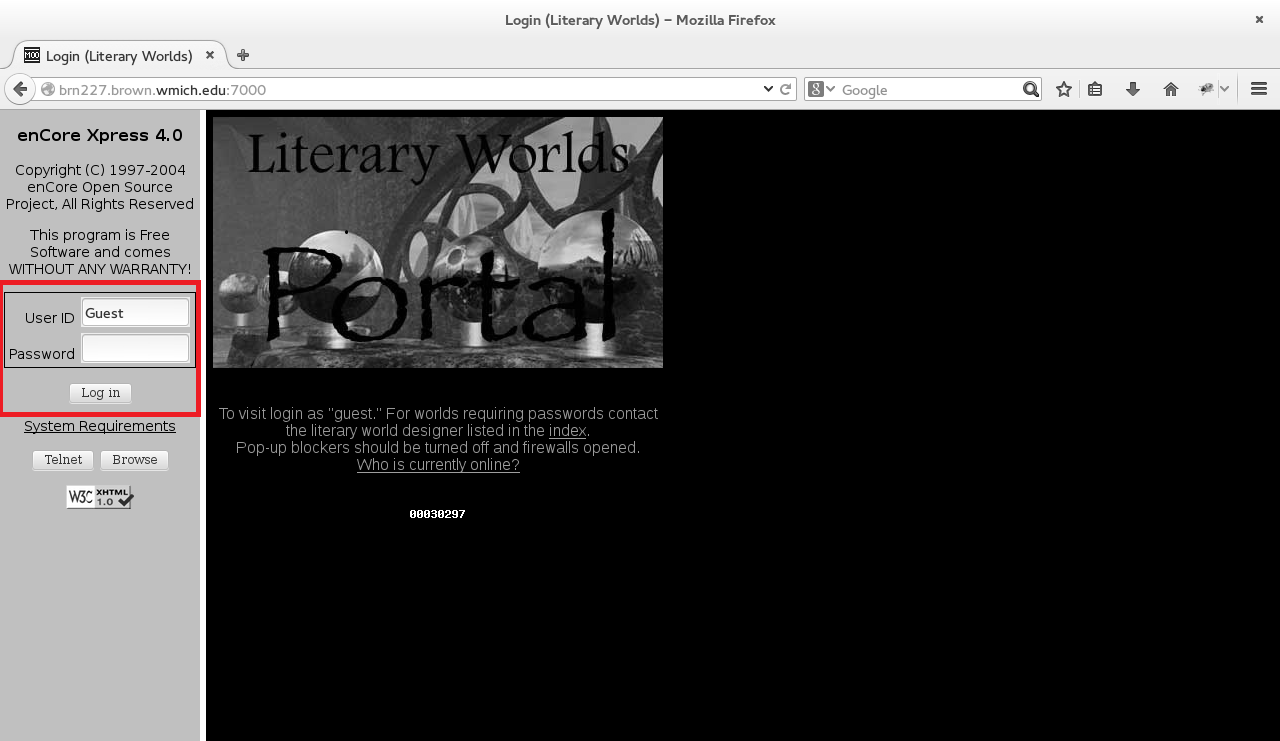
\includegraphics[width=\textwidth,height=\textheight,keepaspectratio]{01_LogIn_GRAY.png}
  \end{centering}
}

\frame{\frametitle{Example}
  \begin{centering}
  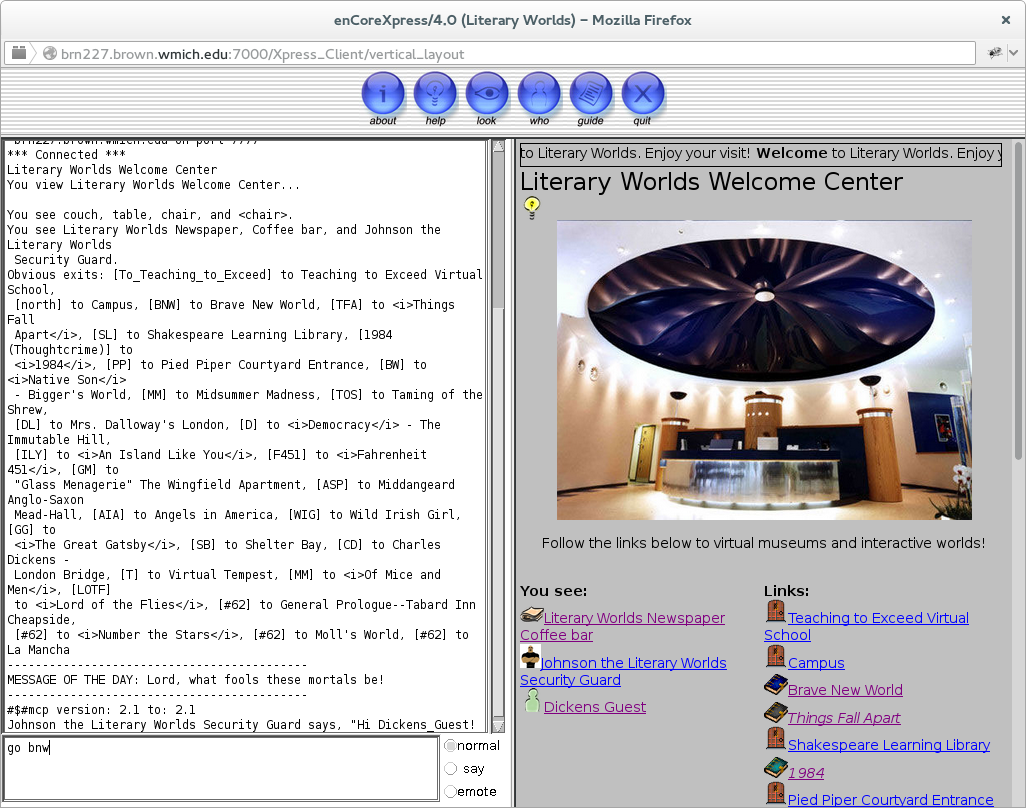
\includegraphics[width=\textwidth,height=\textheight,keepaspectratio]{01_gobnw.png}
  \end{centering}
}

\frame{\frametitle{Example}
  \begin{centering}
  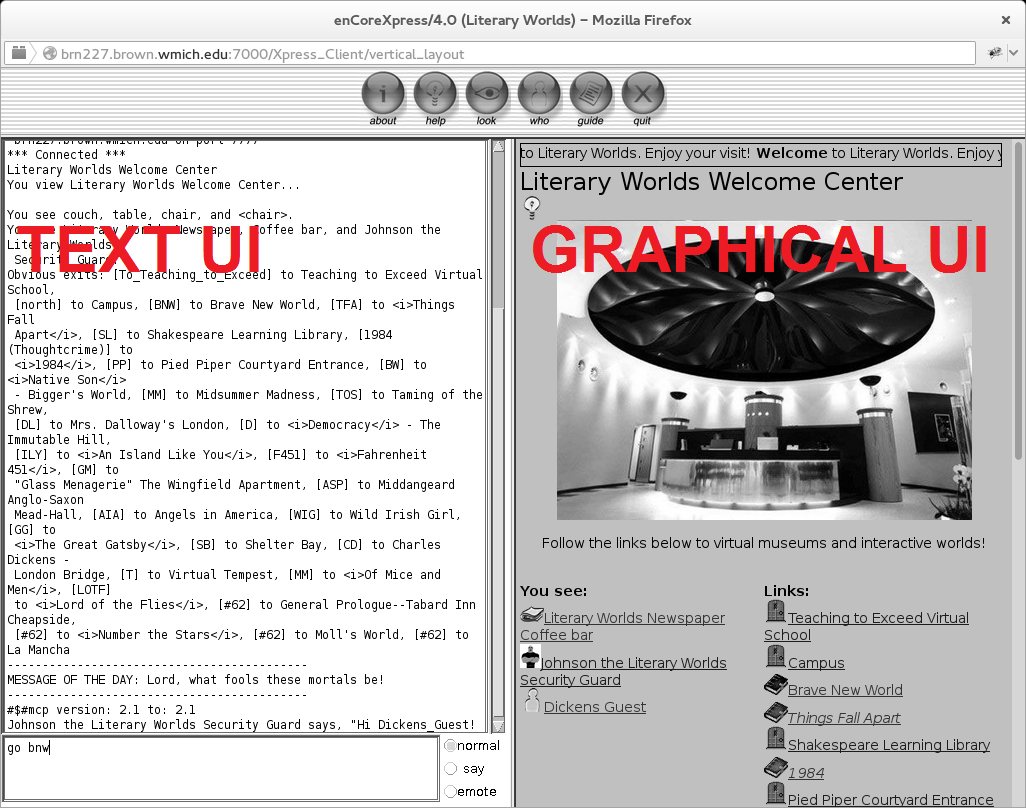
\includegraphics[width=\textwidth,height=\textheight,keepaspectratio]{01_gobnw_ui.png}
  \end{centering}
}

\frame{\frametitle{Example}
  \begin{centering}
  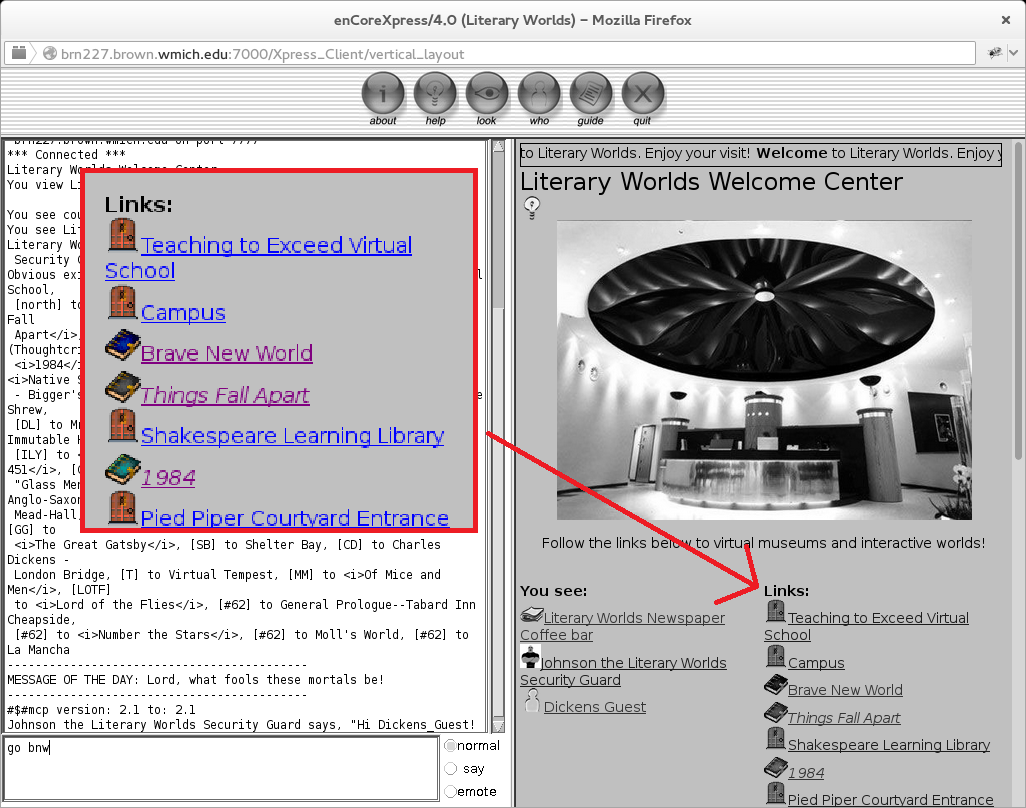
\includegraphics[width=\textwidth,height=\textheight,keepaspectratio]{01_gobnw_Links.png}
  \end{centering}
}

\frame{\frametitle{Example}
  \begin{centering}
  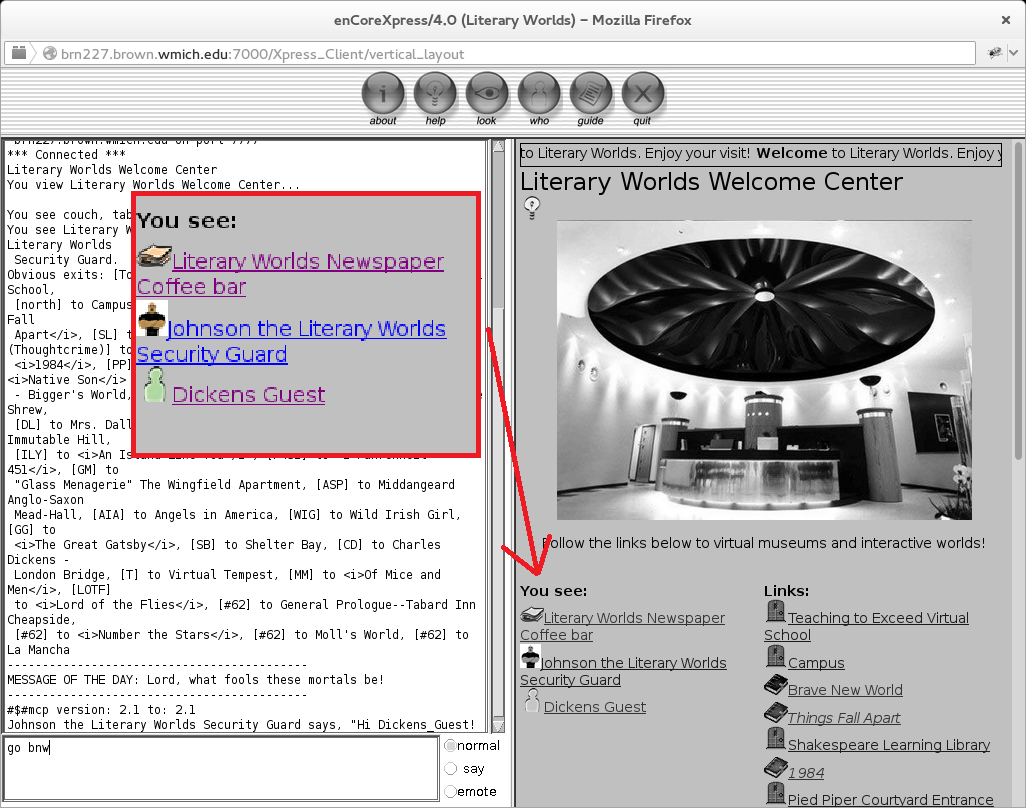
\includegraphics[width=\textwidth,height=\textheight,keepaspectratio]{01_gobnw_Objs.png}
  \end{centering}
}

\frame{\frametitle{Example}
  \begin{centering}
  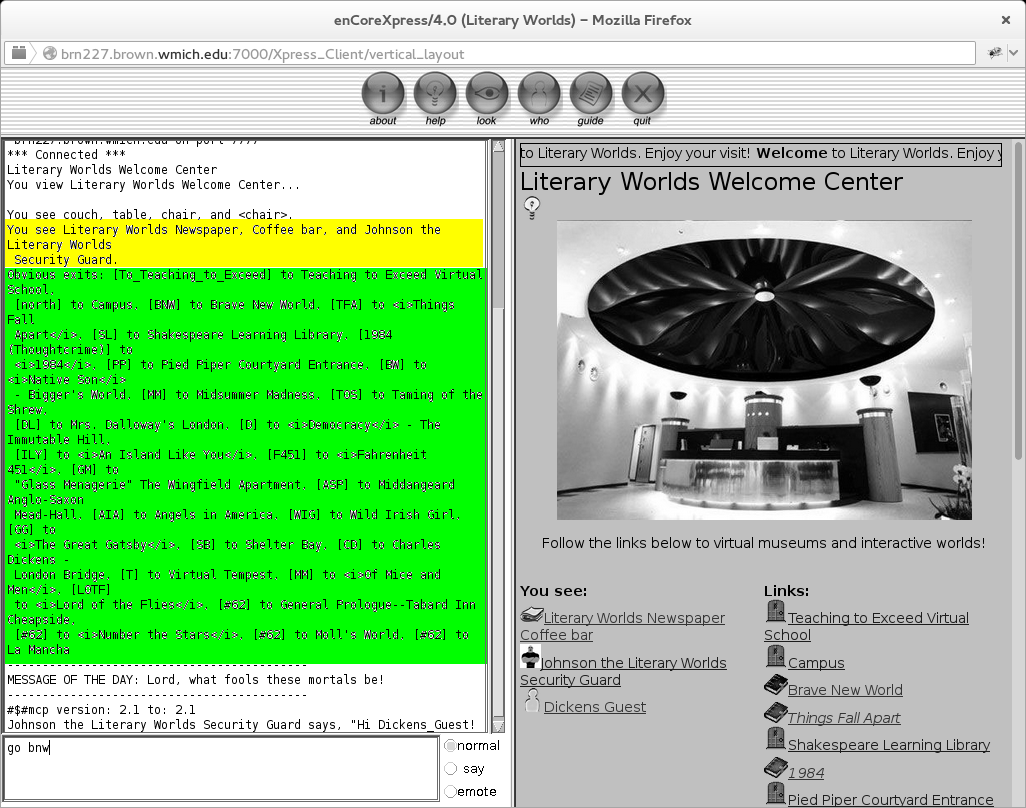
\includegraphics[width=\textwidth,height=\textheight,keepaspectratio]{01_gobnw_telnet.png}
  \end{centering}
}

\frame{\frametitle{Example}
  \begin{centering}
  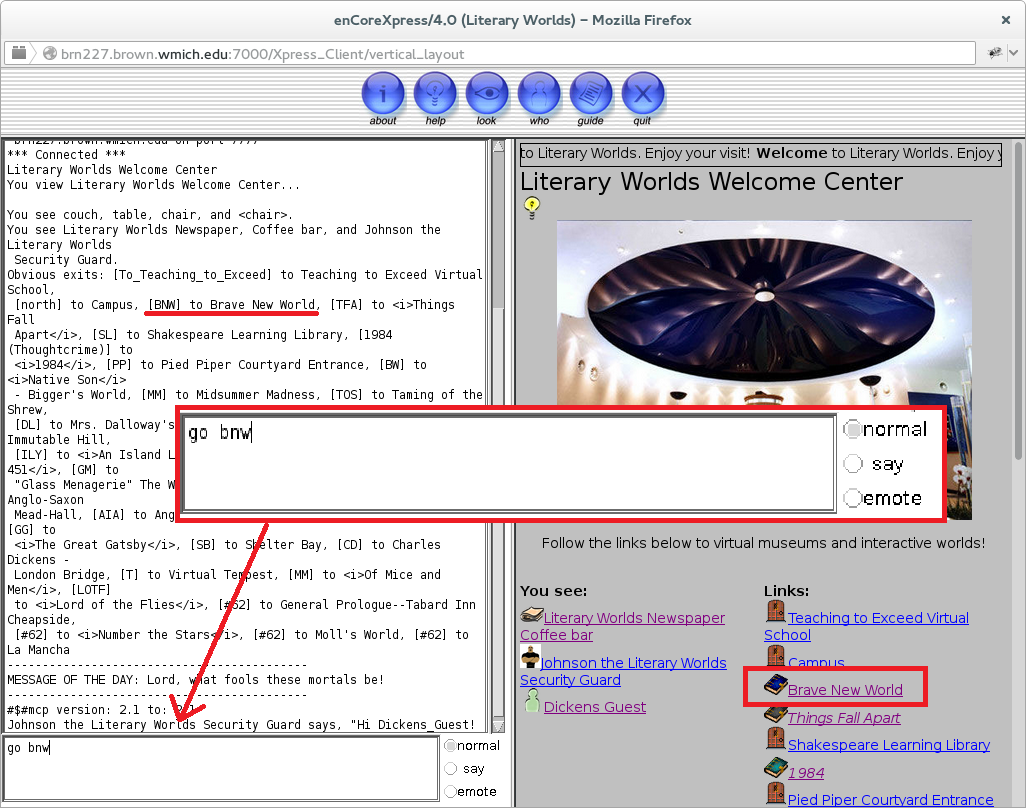
\includegraphics[width=\textwidth,height=\textheight,keepaspectratio]{01_gobnw_cmd.png}
  \end{centering}
}

\frame{\frametitle{Example}
  \begin{centering}
  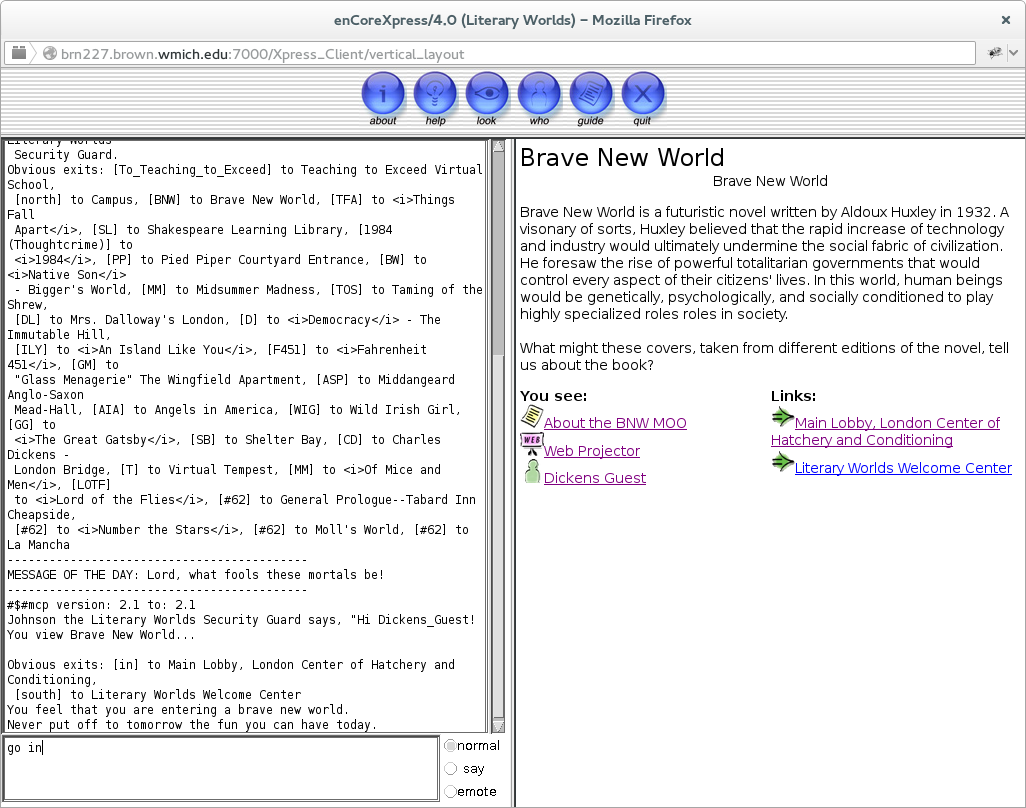
\includegraphics[width=\textwidth,height=\textheight,keepaspectratio]{02_goin.png}
  \end{centering}
}

\frame{\frametitle{Example}
  \begin{centering}
  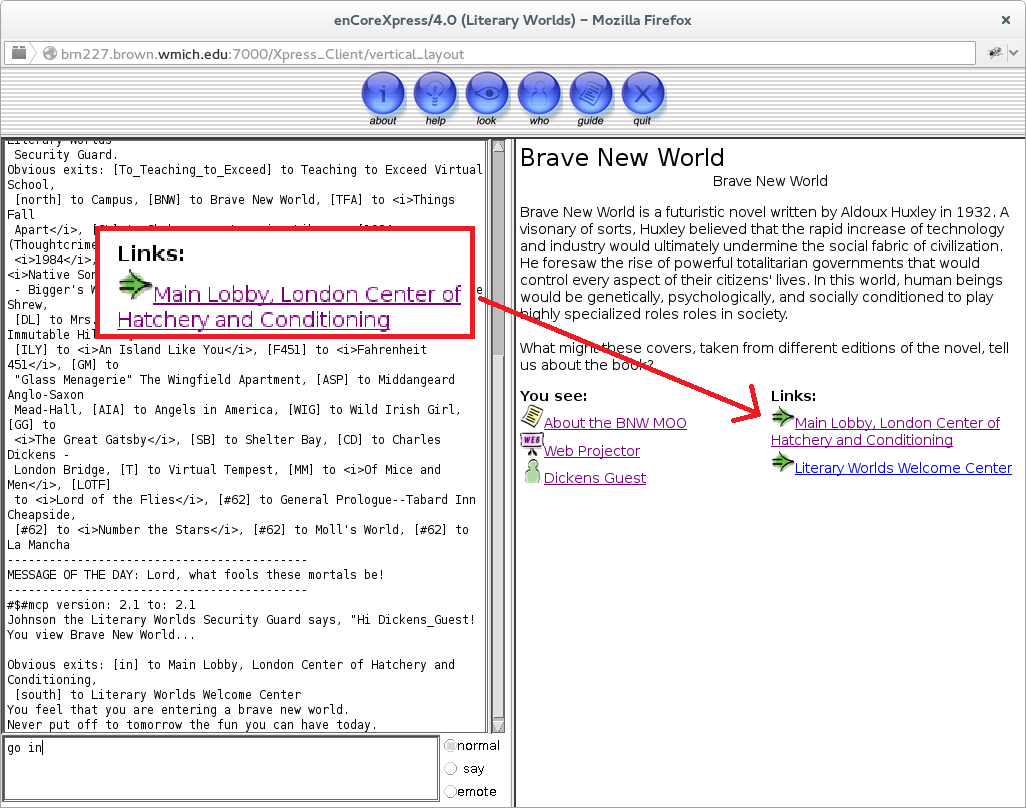
\includegraphics[width=\textwidth,height=\textheight,keepaspectratio]{02_goin_red.png}
  \end{centering}
}

\frame{\frametitle{Example}
  \begin{centering}
  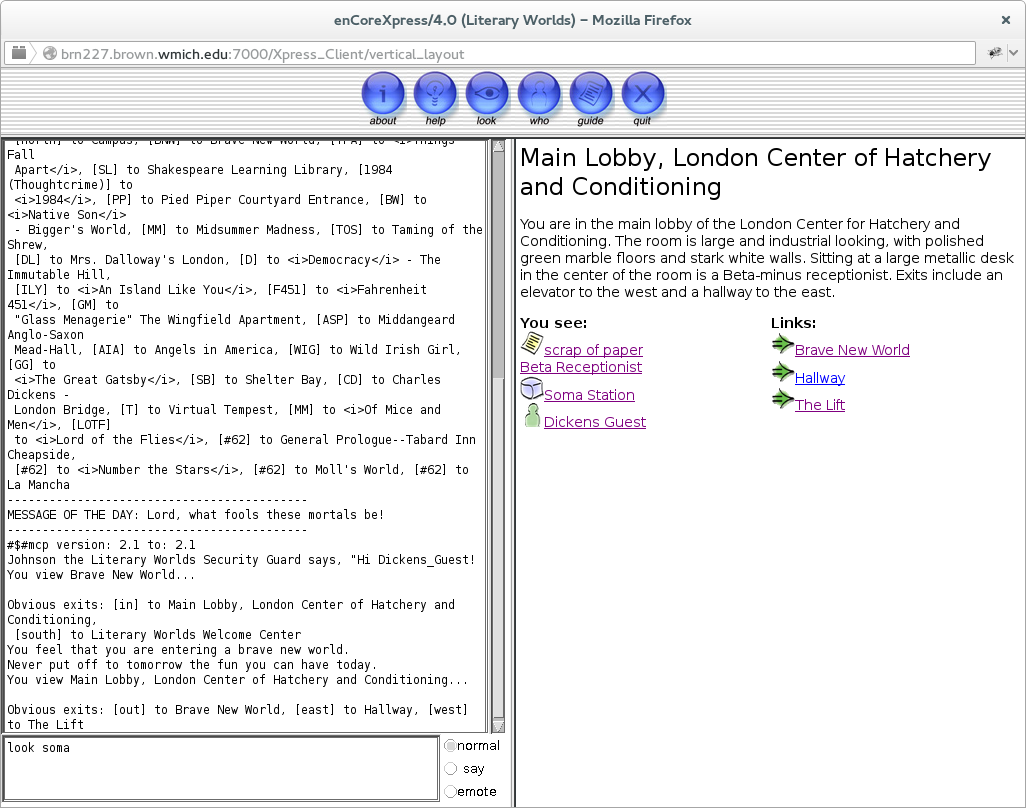
\includegraphics[width=\textwidth,height=\textheight,keepaspectratio]{03_looksoma.png}
  \end{centering}
}

\frame{\frametitle{Example}
  \begin{centering}
  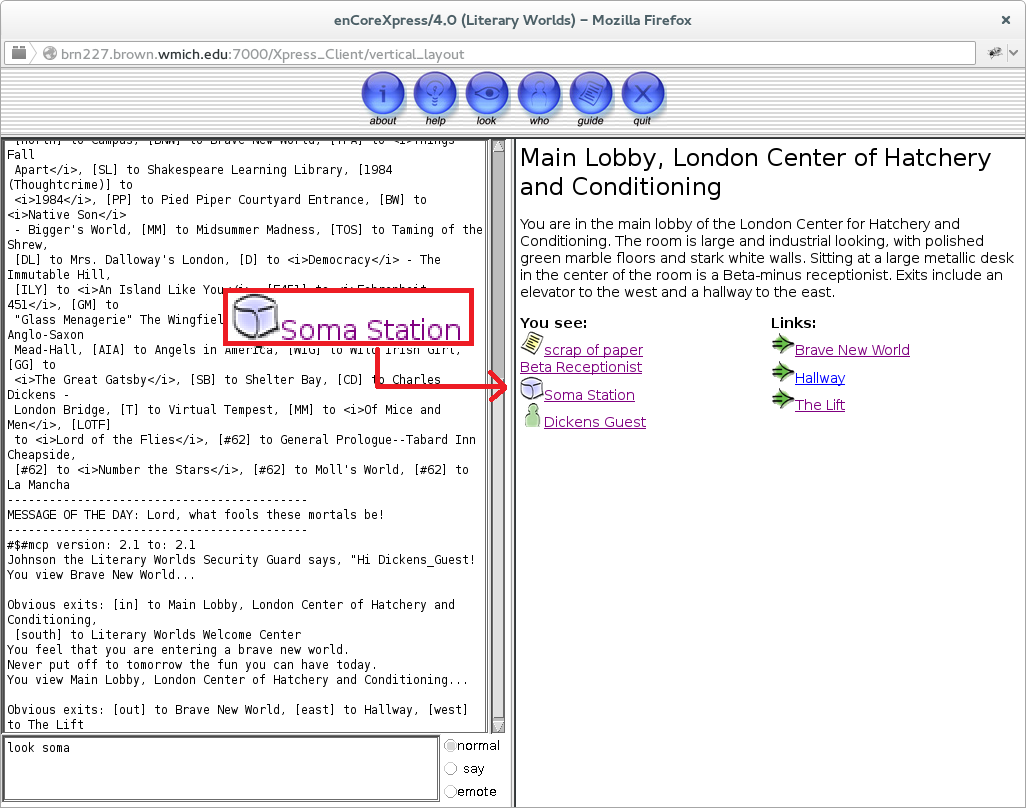
\includegraphics[width=\textwidth,height=\textheight,keepaspectratio]{03_looksoma_red.png}
  \end{centering}
}

\frame{\frametitle{Example}
  \begin{centering}
  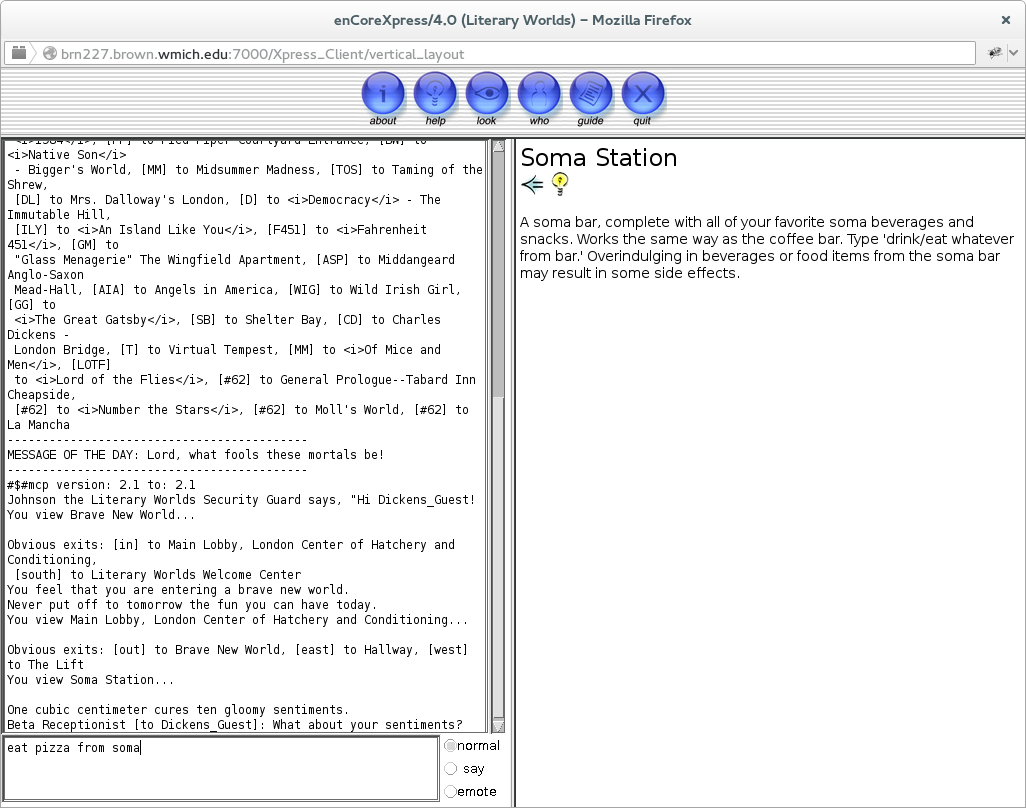
\includegraphics[width=\textwidth,height=\textheight,keepaspectratio]{04_eatpizzafromsoma.png}
  \end{centering}
}

\frame{\frametitle{Example}
  \begin{centering}
  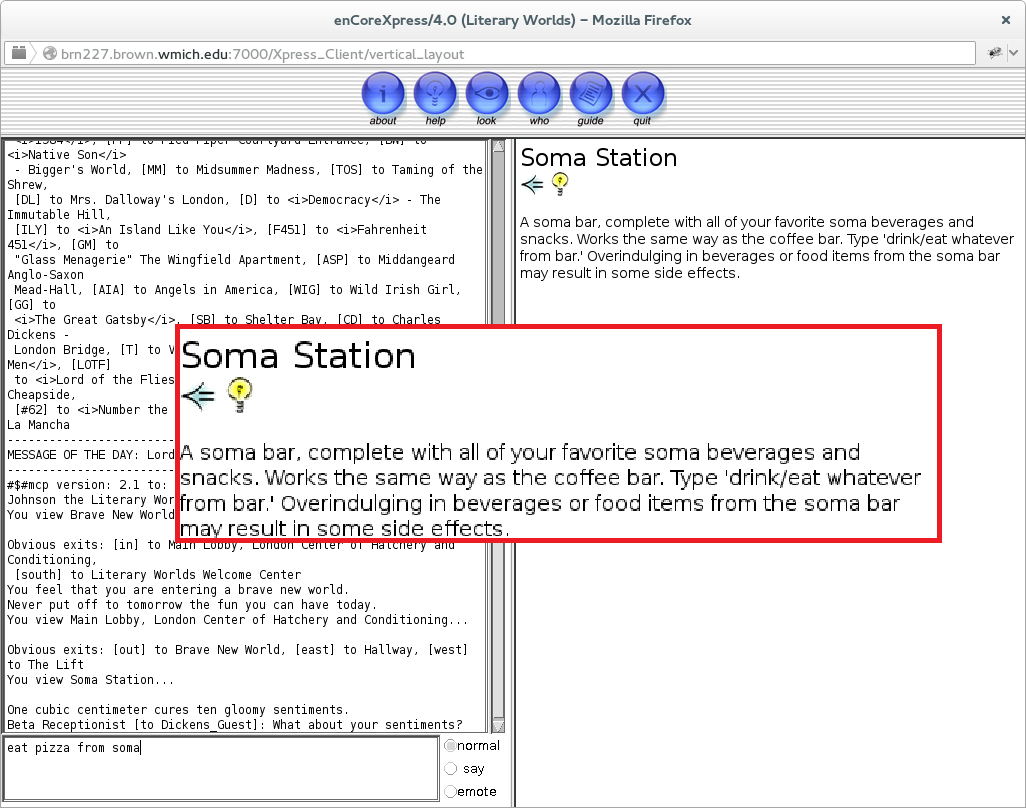
\includegraphics[width=\textwidth,height=\textheight,keepaspectratio]{04_eatpizzafromsoma_red1.png}
  \end{centering}
}

\frame{\frametitle{Example}
  \begin{centering}
  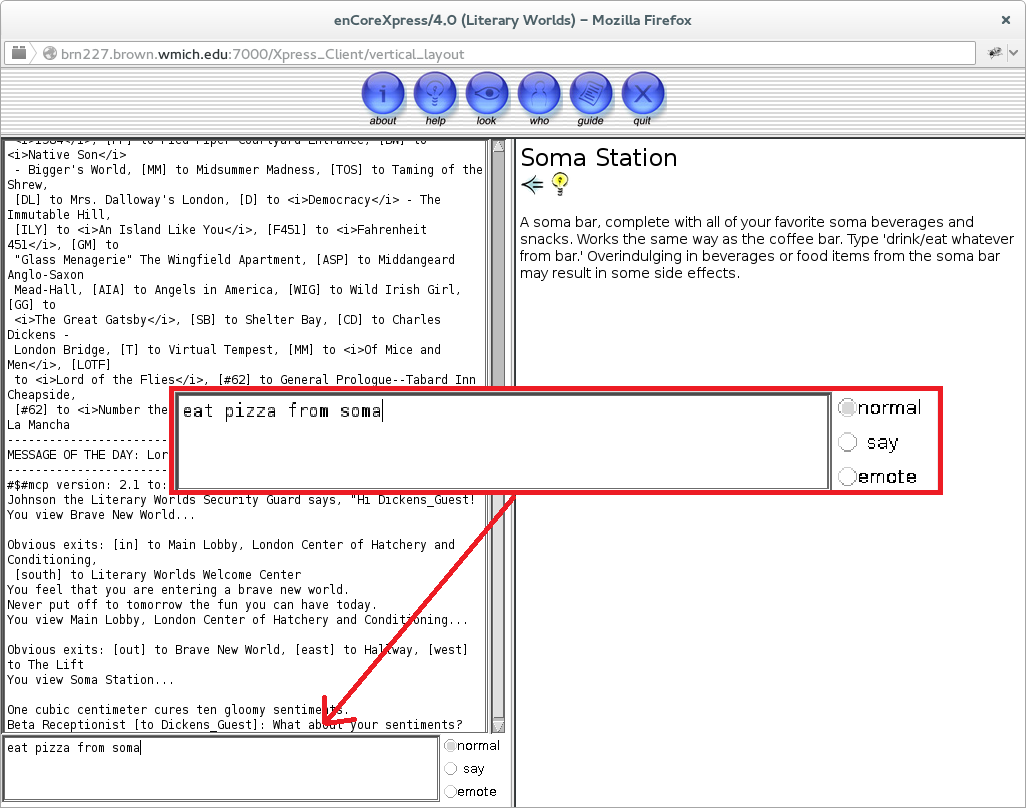
\includegraphics[width=\textwidth,height=\textheight,keepaspectratio]{04_eatpizzafromsoma_red2.png}
  \end{centering}
}

\frame{\frametitle{Example}
  \begin{centering}
  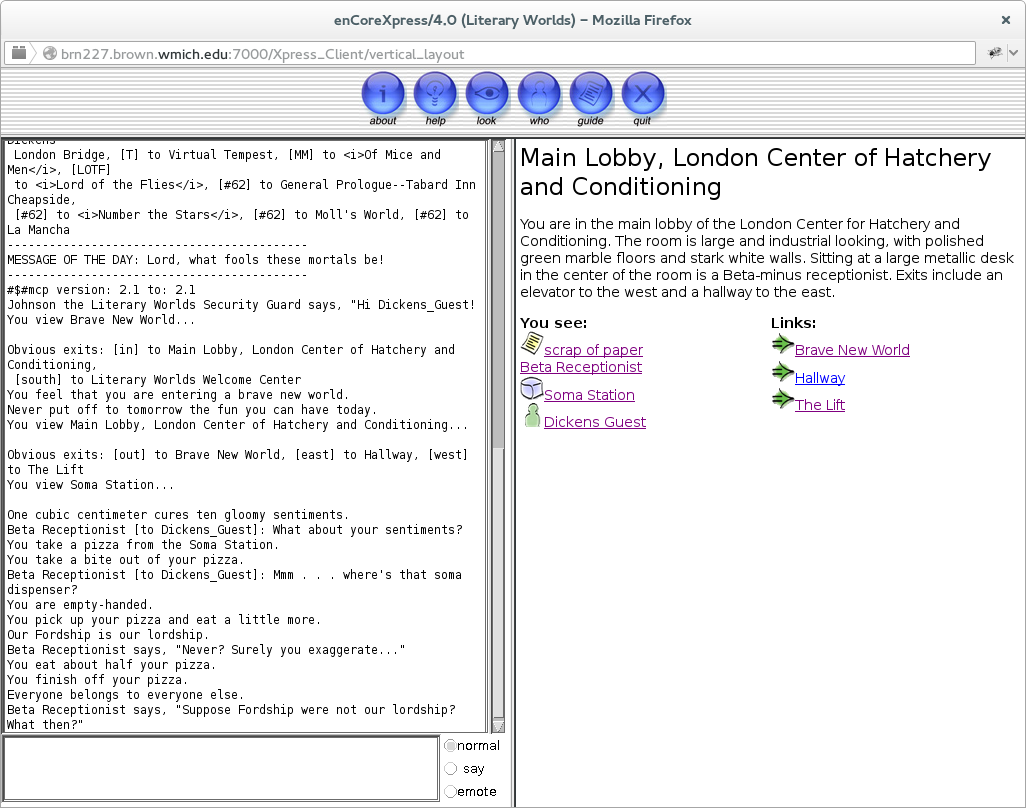
\includegraphics[width=\textwidth,height=\textheight,keepaspectratio]{06_pizzadone.png}
  \end{centering}
}

\frame{\frametitle{Example}
  \begin{centering}
  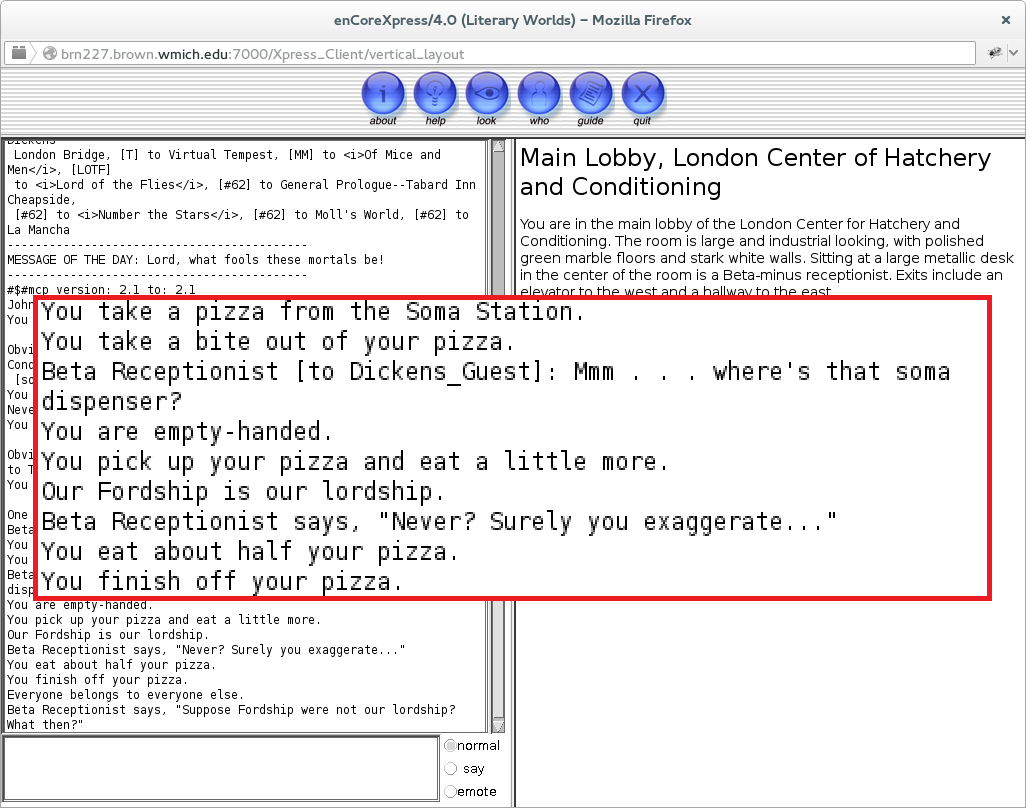
\includegraphics[width=\textwidth,height=\textheight,keepaspectratio]{06_pizzadone_red.png}
  \end{centering}
}

\frame{\frametitle{Example}
  \begin{centering}
  GUI only and Text only modes are available
  
  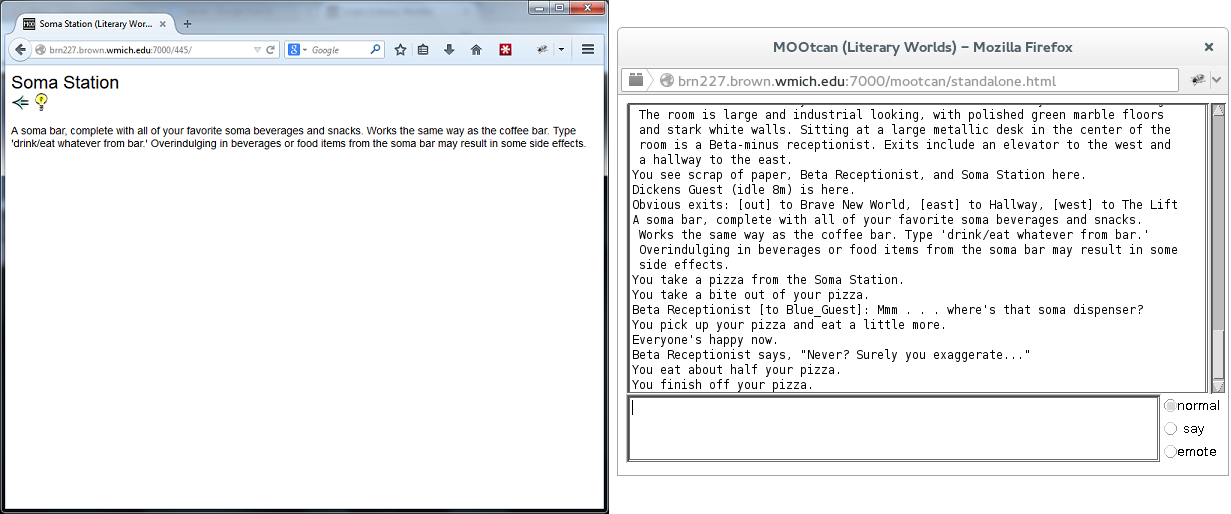
\includegraphics[width=\textwidth,height=\textheight,keepaspectratio]{GUInTUIOnly.png}
  \end{centering}
}

\frame{\frametitle{Only The Basics}
  \begin{centering}
  \begin{itemize}
    \item Entire classrooms with many users
    \item Log on a characters from the text
    \item Village of Umofia created by Dr. Allen Webb
  \end{itemize}
   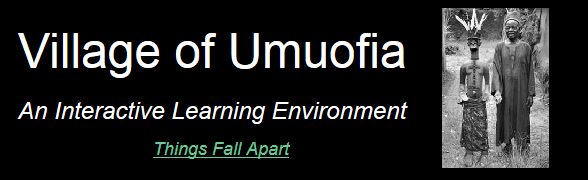
\includegraphics[width=\textwidth,height=\textheight,keepaspectratio]{vou_logo.png}
  \end{centering}
}

\frame{\frametitle{Village of Umuofia}
\begin{centering}

\begin{itemize}
\item Users may use this environment in a variety of ways
\begin{itemize}
\item A gallery of images of Igbo village that show life and traditional West African music
\item An interactive space for live action role play activities based on the novel (Things Fall Apart)
\end{itemize}
\end{itemize}
\end{centering}
}

\frame{\frametitle{Village of Umuofia}
\begin{centering}

\begin{itemize}
\item Literary Worlds allows users to further understand the novel's characters, environments, and themes
\end{itemize}
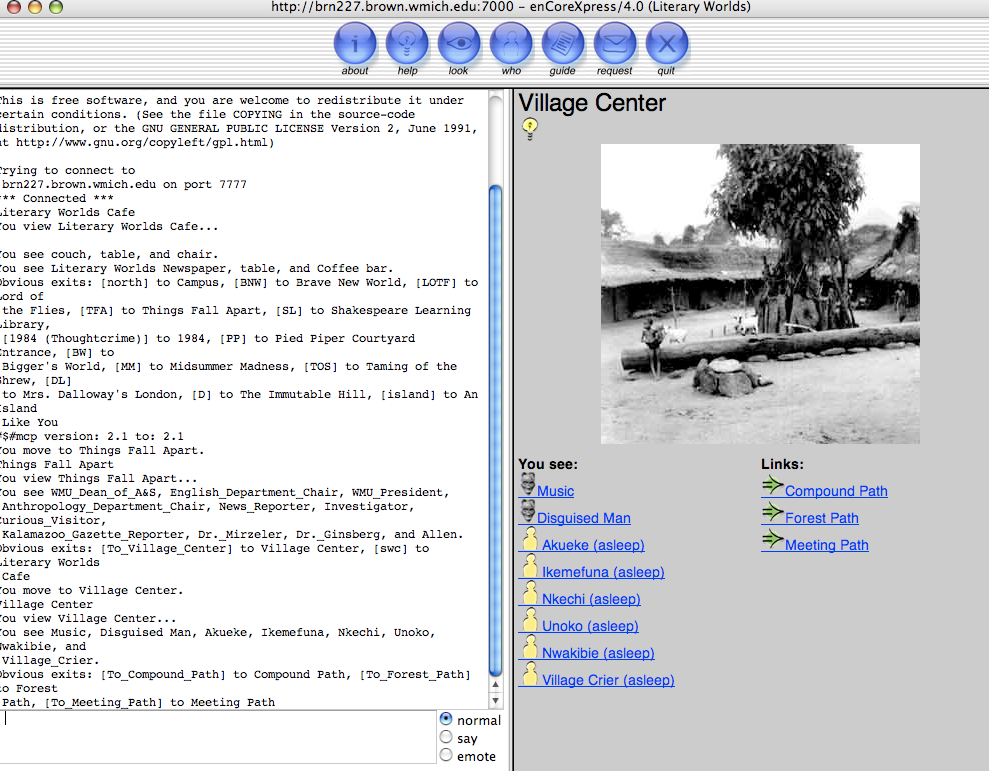
\includegraphics[width=0.75\textwidth,height=\textheight,keepaspectratio,center]{village.png}
\end{centering}
}

\section{Introduction}

\frame{\frametitle{Current Technology}
  \begin{itemize}
    \item LambdaMOO 
      \begin{itemize}
      \item A MUD server software package
      \item Provides telnet interface
      \end{itemize}
    \item enCore Xpress
      \begin{itemize}
      \item A MOO database and interface
      \item provides HTML interface
      \end{itemize}
  \end{itemize}
}


\frame{\frametitle{enCore Client-Server Diagram}
  \begin{centering}
  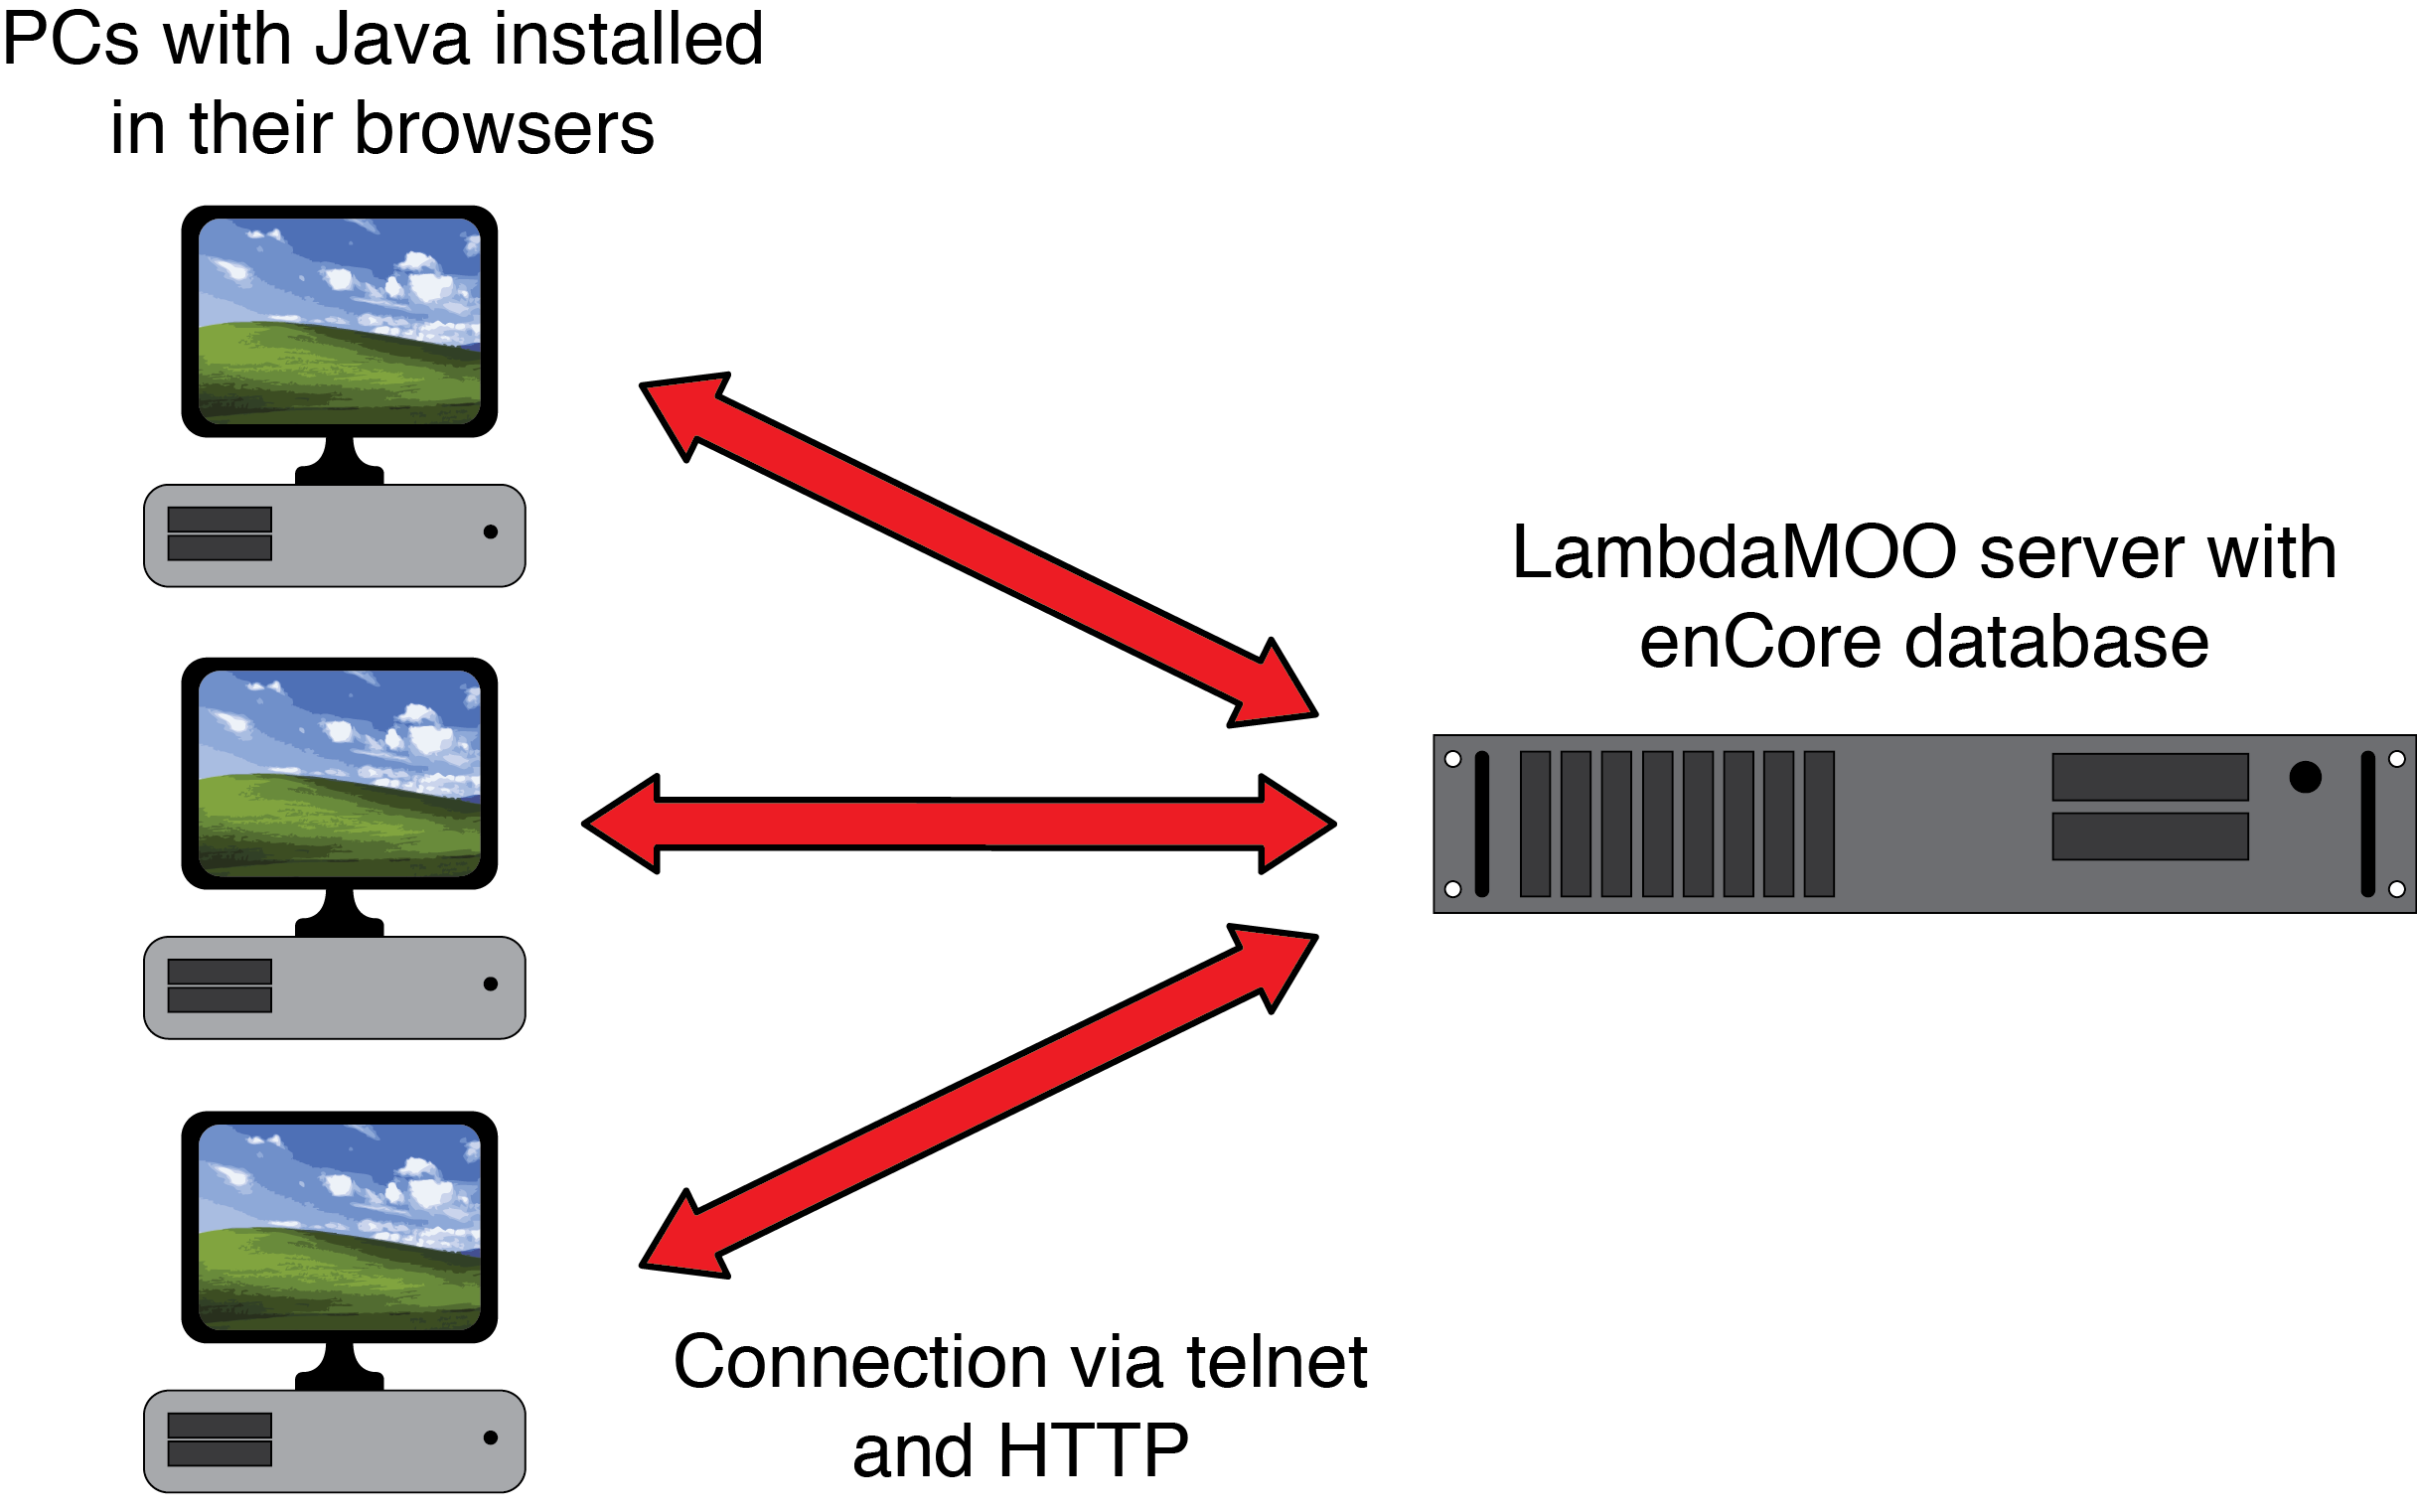
\includegraphics[width=\textwidth,height=\textheight,keepaspectratio]{TelnetDiagram.png}
  \end{centering}
}


\frame{\frametitle{Problems - Java}
  \begin{centering}

  \centerline{
  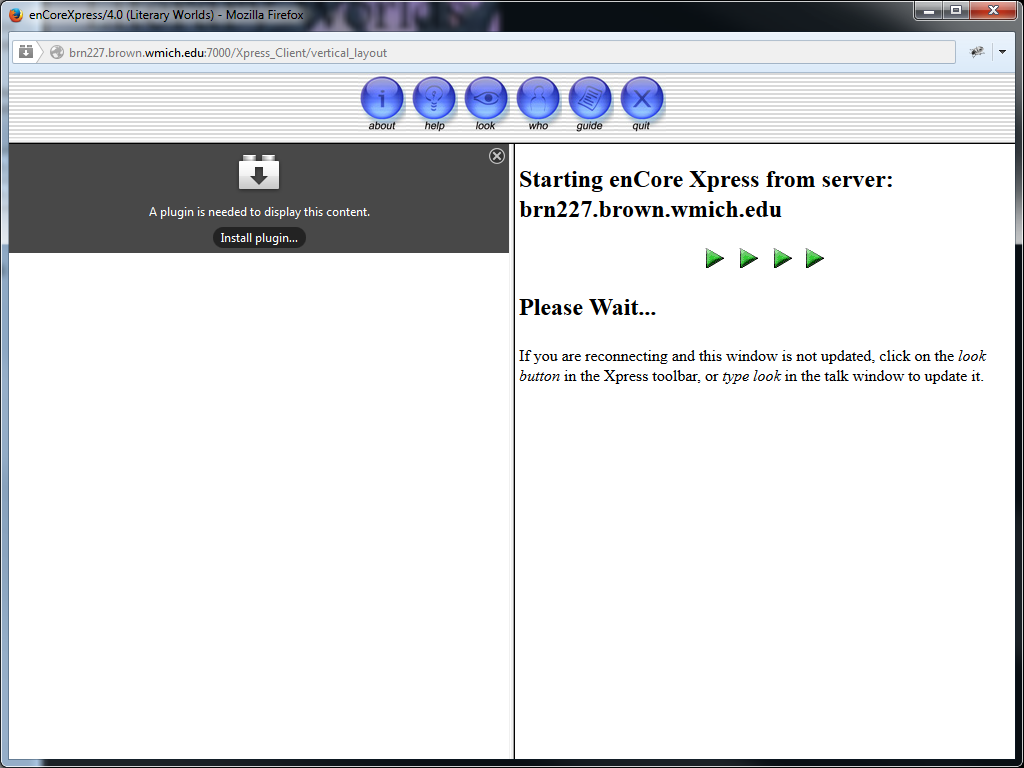
\includegraphics[width=\textwidth,height=0.8\textheight,keepaspectratio]{PlugInNeeded.png}}
  \end{centering}
}


\frame{\frametitle{Things to Keep in Mind}
  \begin{centering}
  \begin{itemize}
  \item Over 20 virtual worlds currently make up Literary Worlds
  \item Any replacement interface needs to keep the virtual worlds functioning, as they are.
    \begin{itemize}
    \item No change to the current server
    \end{itemize}
  \item Need to remove the Java dependency
  \end{itemize}
  \end{centering}
}

\section{Design Decisions}
\frame{\frametitle{New Client-Server Design}
  \begin{itemize}
    \item Not possible for javascript in browser to use Telnet
    \item Therefore, we need an intermediate server to handle Telnet
    \item Must support concurrent users and handle asynchronous events
    \item Must keep the graphical and text modes in sync as the user moves in the world
  \end{itemize}
}

%
%\frame{\frametitle{Design Decisions}
%  \begin{itemize}
%  \item Text Mode
%    \begin{itemize}
%      \item Client side Javascript MUD client
%      \item This is reason an intermediary server is needed, to handle the telnet connection on behalf of each client.
%    \end{itemize}
%  \item Graphical Mode
%    \begin{itemize}
%      \item This work is already done in enCore Xpress, there is no need to reinvent it.
%      \item The new web application will simply need to serve the existing enCore Xpress interface in a coherent way.
%    \end{itemize}
%  \end{itemize}
%}

\frame{\frametitle{New Client Technology}
  % Backbone, Bootstrap, Socket.io, Coffeescript
  
\includegraphics[width=\textwidth, height=\textheight,keepaspectratio]{clientstack.png}
  \begin{itemize}
  \item Socket.io
    \begin{itemize}
      \item A websocket library for realtime communication
    \end{itemize}
  \item Backbone.js
    \begin{itemize}
      \item A templating library for Javascript web applications
    \end{itemize}
  \item Bootstrap
    \begin{itemize}
    \item A popular frontend layout toolkit
    \item Provides grid system for responsive design
    \end{itemize}
  \item Coffeescript
    \begin{itemize}
      \item A simple language that translates to Javascript
    \end{itemize}
  \end{itemize}
}

\frame{\frametitle{Intermediate Server Technology}
  % Node.JS here
  
\includegraphics[width=0.66\textwidth, height=\textheight,keepaspectratio,center]{serverstack.png}
  \begin{itemize}
  \item Node.js
    \begin{itemize}
      \item server side runtime for Javascript built on Google's V8
    \end{itemize}
  \item Express
    \begin{itemize}
      \item Web app framework for Node.js
      \item provides tools for REST, URL routing, cookies, etc.
    \end{itemize}
    \item Socket.io
      \begin{itemize}
        \item Websocket server
      \end{itemize}
    \item Request
      \begin{itemize}
      \item simple HTTP request library
      \end{itemize}
    \item Cheerio
      \begin{itemize}
      \item provides a subset of jQuery on a server
      \end{itemize}
    \item CoffeeScript
    
  \end{itemize}
}

\frame{\frametitle{Syncing User Experience}
\begin{itemize}
  \item enCore uses a cookie system to sync graphical and text interfaces
  \item New graphical and text interfaces work independently
  \item New client has to hook into old sync system

\end{itemize}
}

\frame{\frametitle{New Client-Server Diagram}
  \begin{centering}
  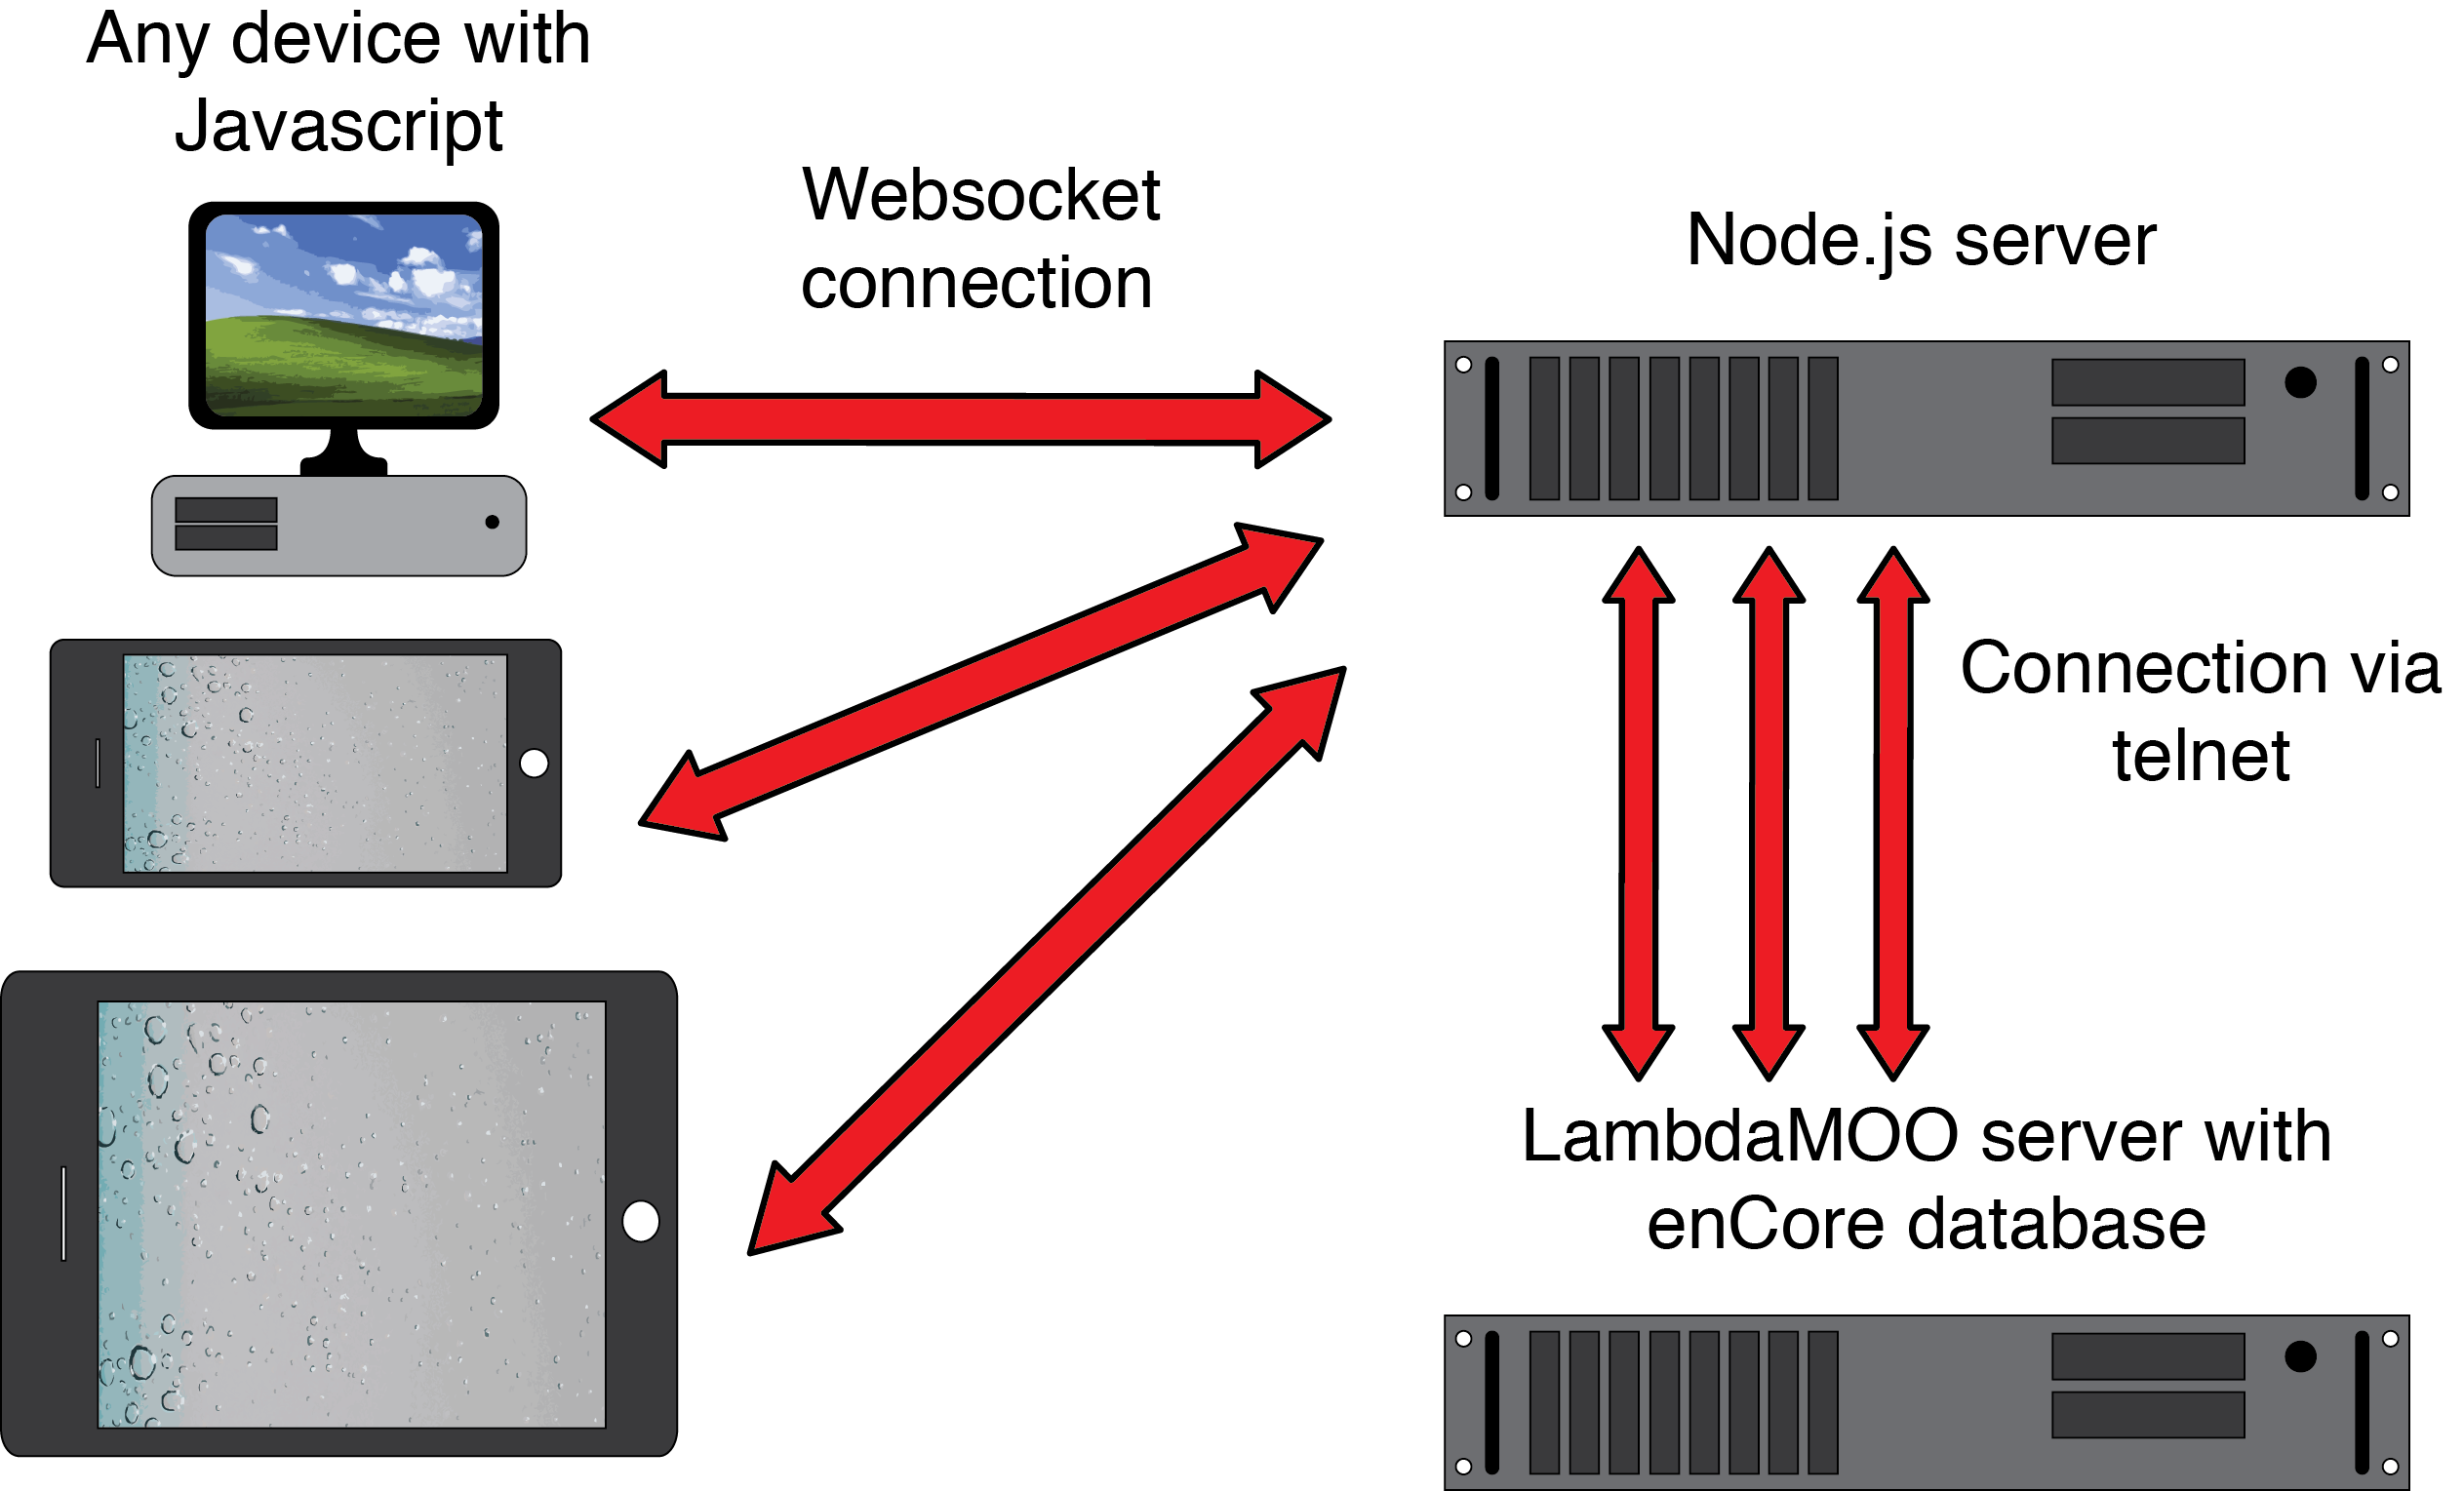
\includegraphics[width=\textwidth,height=\textheight,keepaspectratio]{NodeDiagram.png}
  \end{centering}
}

\section{Implementation}
\frame{\frametitle{New Client Text Interface}
  \begin{centering}
  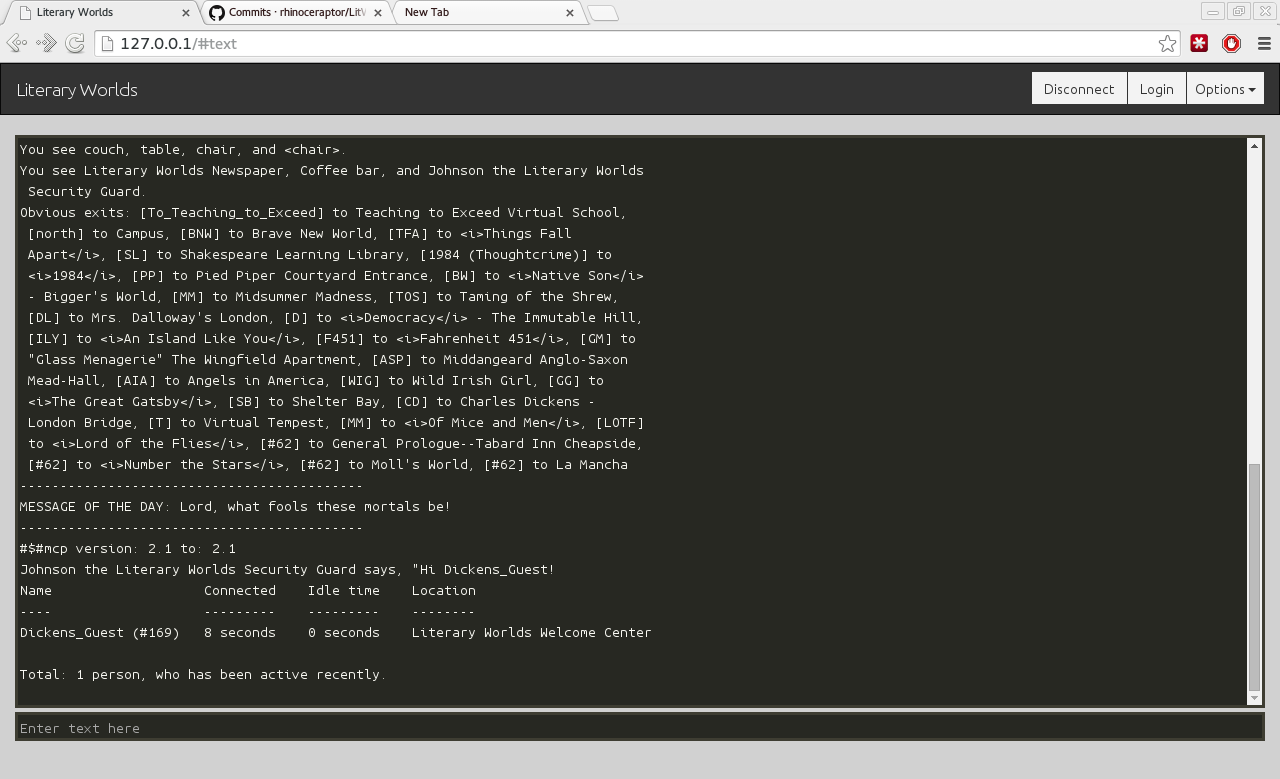
\includegraphics[width=\textwidth,height=\textheight,keepaspectratio]{litworlds_nov_28_text.png}
  \end{centering}
}

\frame{\frametitle{New Client Graphical Interface}
  \begin{centering}
  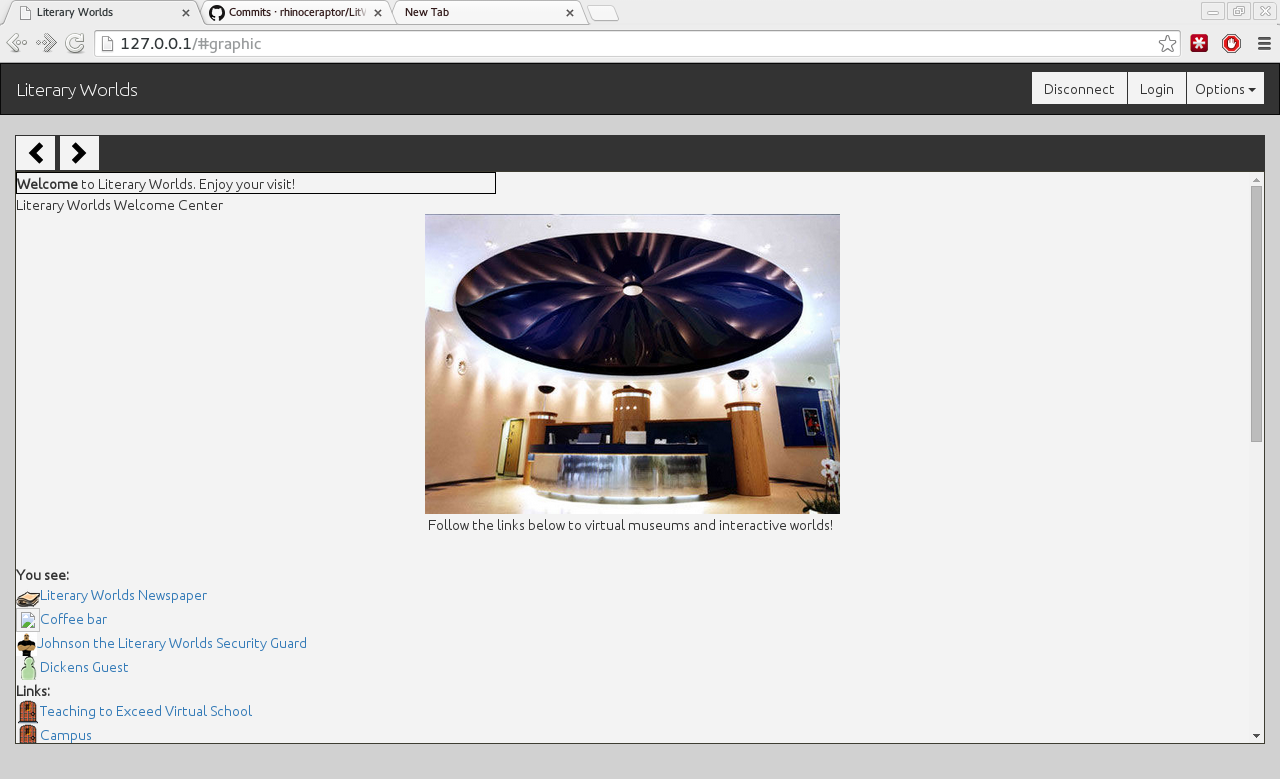
\includegraphics[width=\textwidth,height=\textheight,keepaspectratio]{litworlds_nov_28_graphic.png}
  \end{centering}
}

\frame{\frametitle{New Client Mixed Interface}
  \begin{centering}
  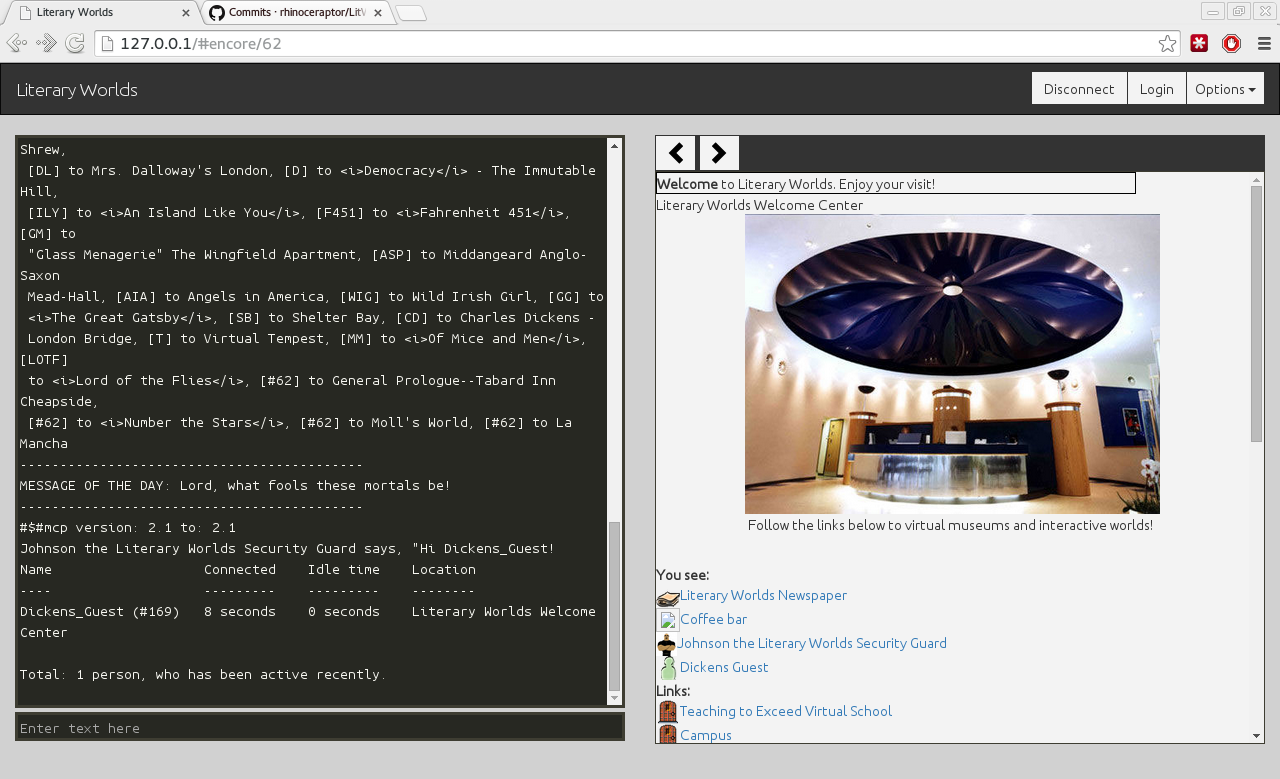
\includegraphics[width=\textwidth,height=\textheight,keepaspectratio]{litworlds_nov_28_mixed.png}
  \end{centering}
}

\frame{\frametitle{Choosing Layout}
  \begin{centering}
  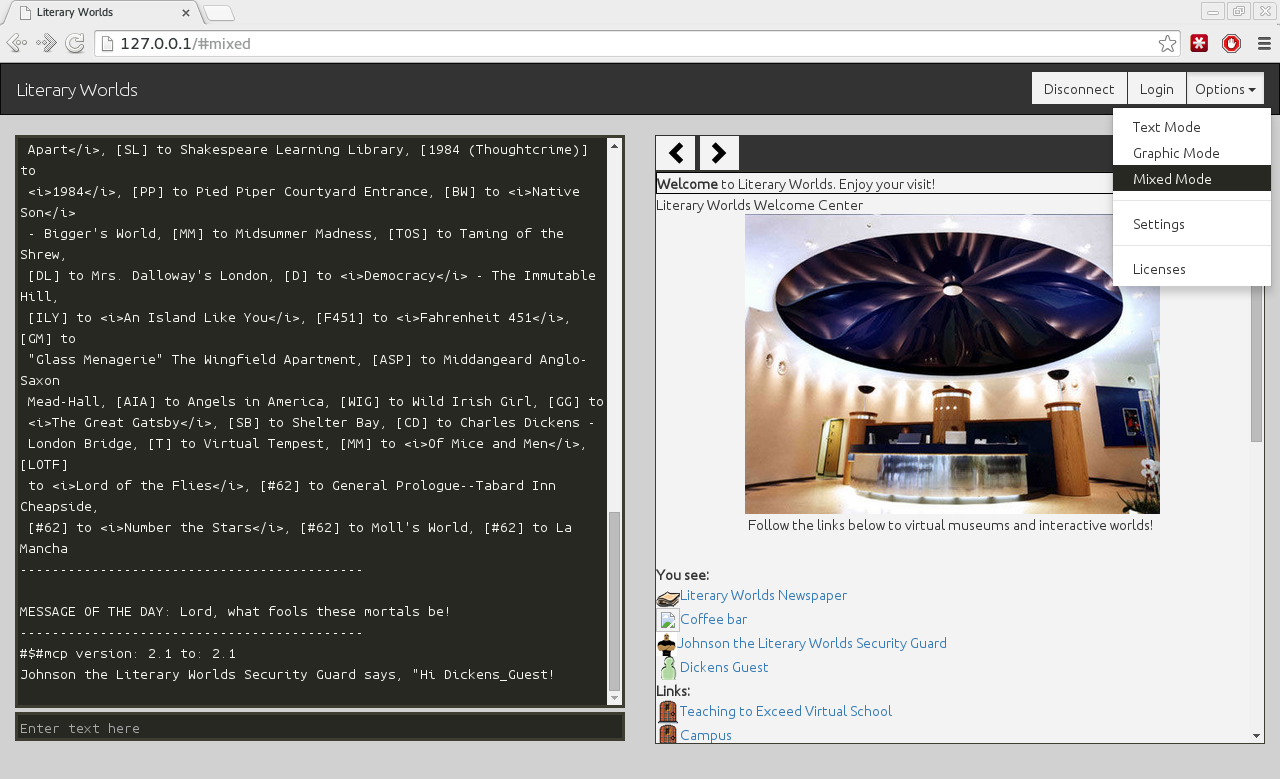
\includegraphics[width=\textwidth,height=\textheight,keepaspectratio]{bootstrap_dropdown.png}
  \end{centering}
}

\frame{\frametitle{HTML sequence}
  \begin{centering}
  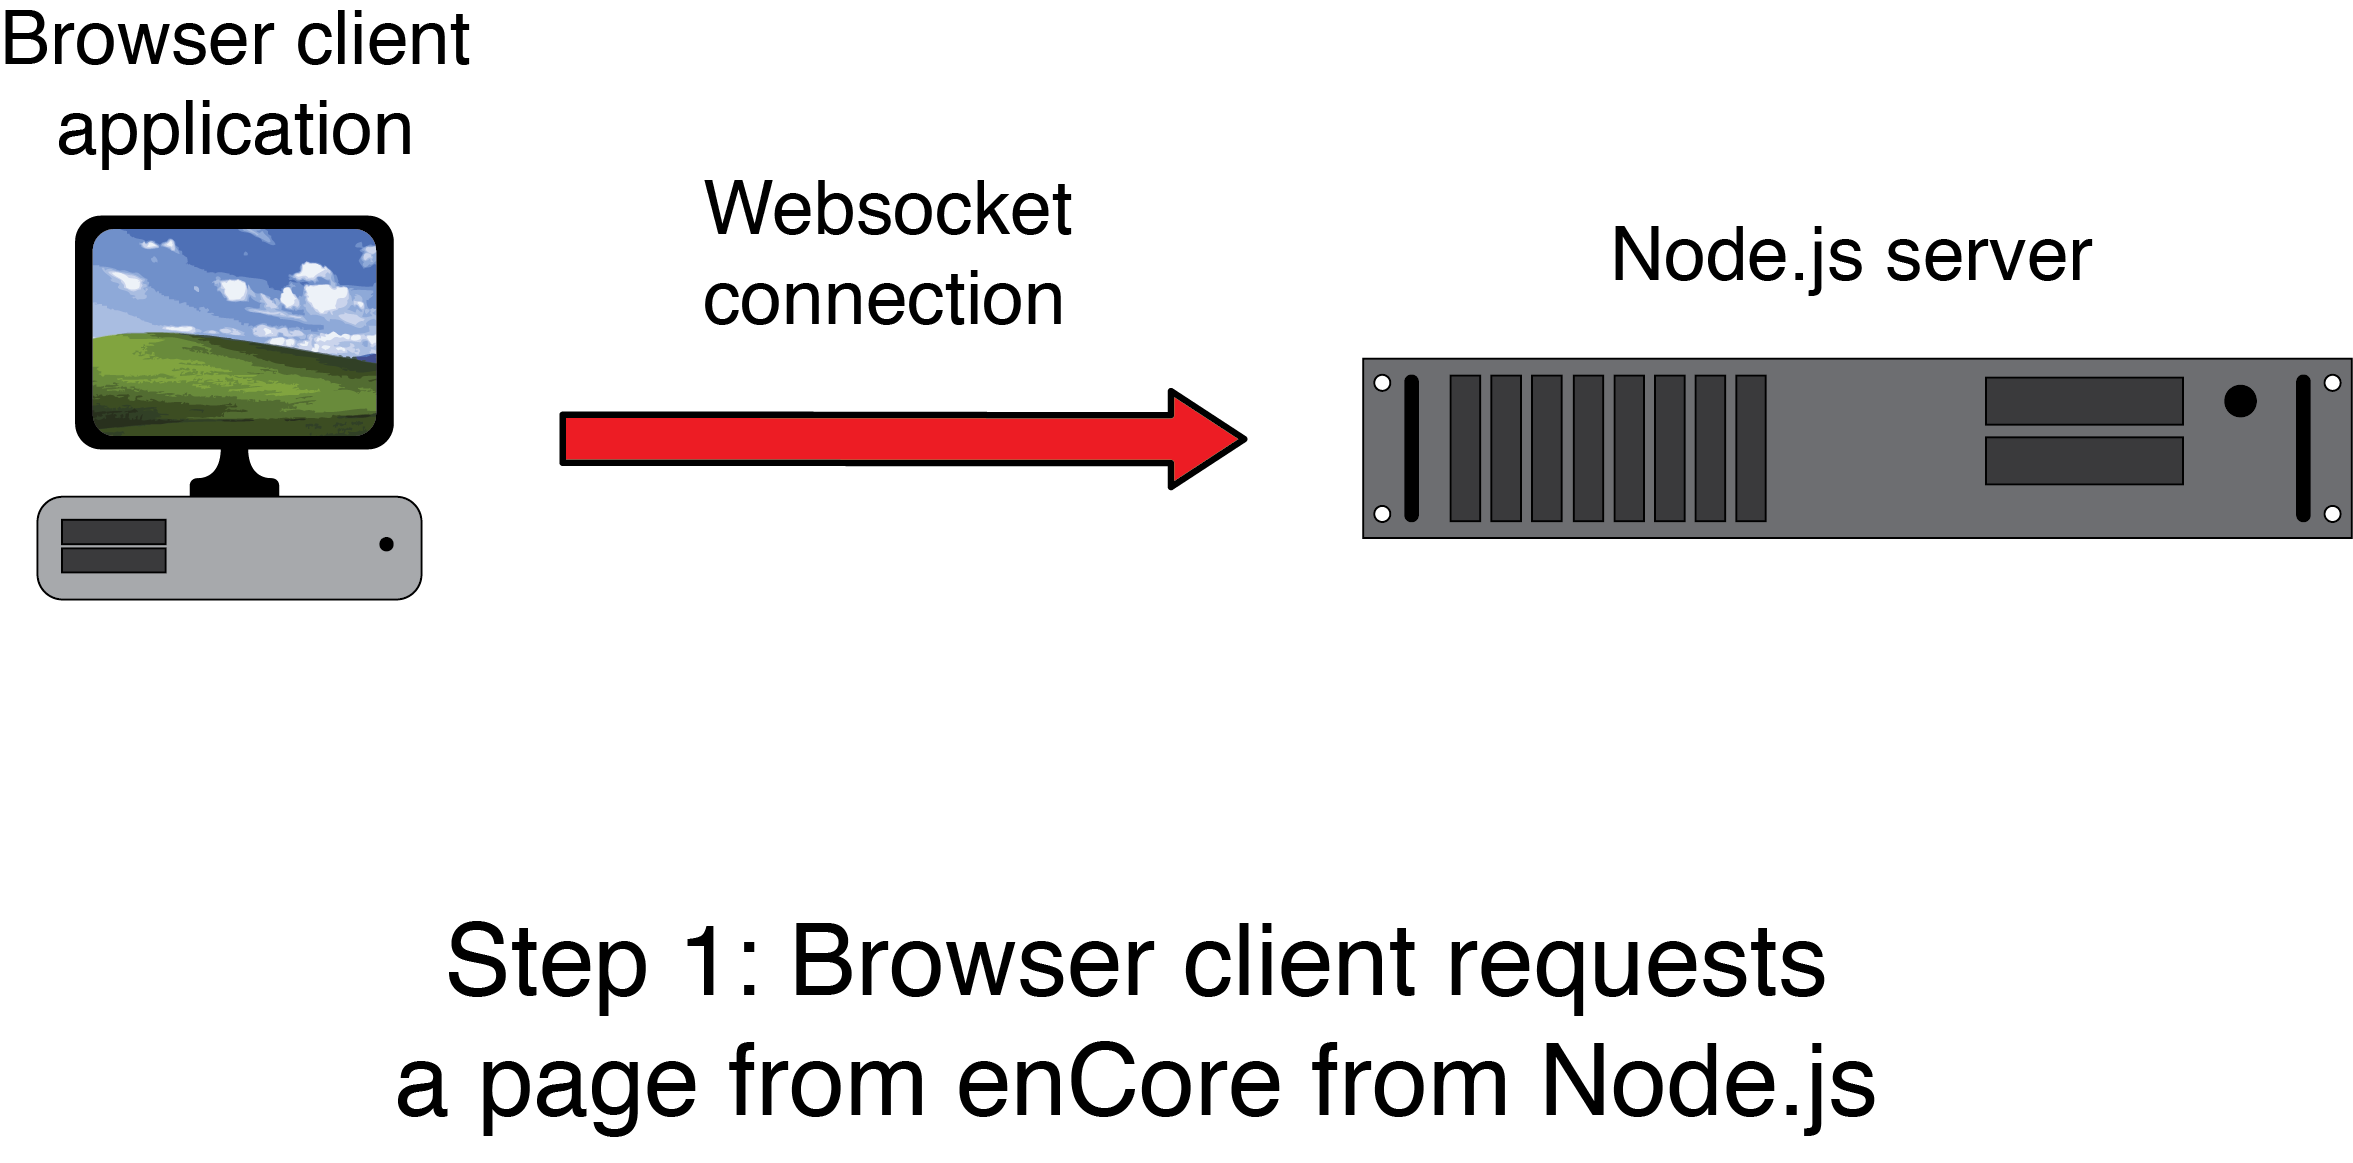
\includegraphics[width=\textwidth,height=\textheight,keepaspectratio]{NodeDiagram_1.png}
  \end{centering}
}

\frame{\frametitle{HTML sequence}
  \begin{centering}
  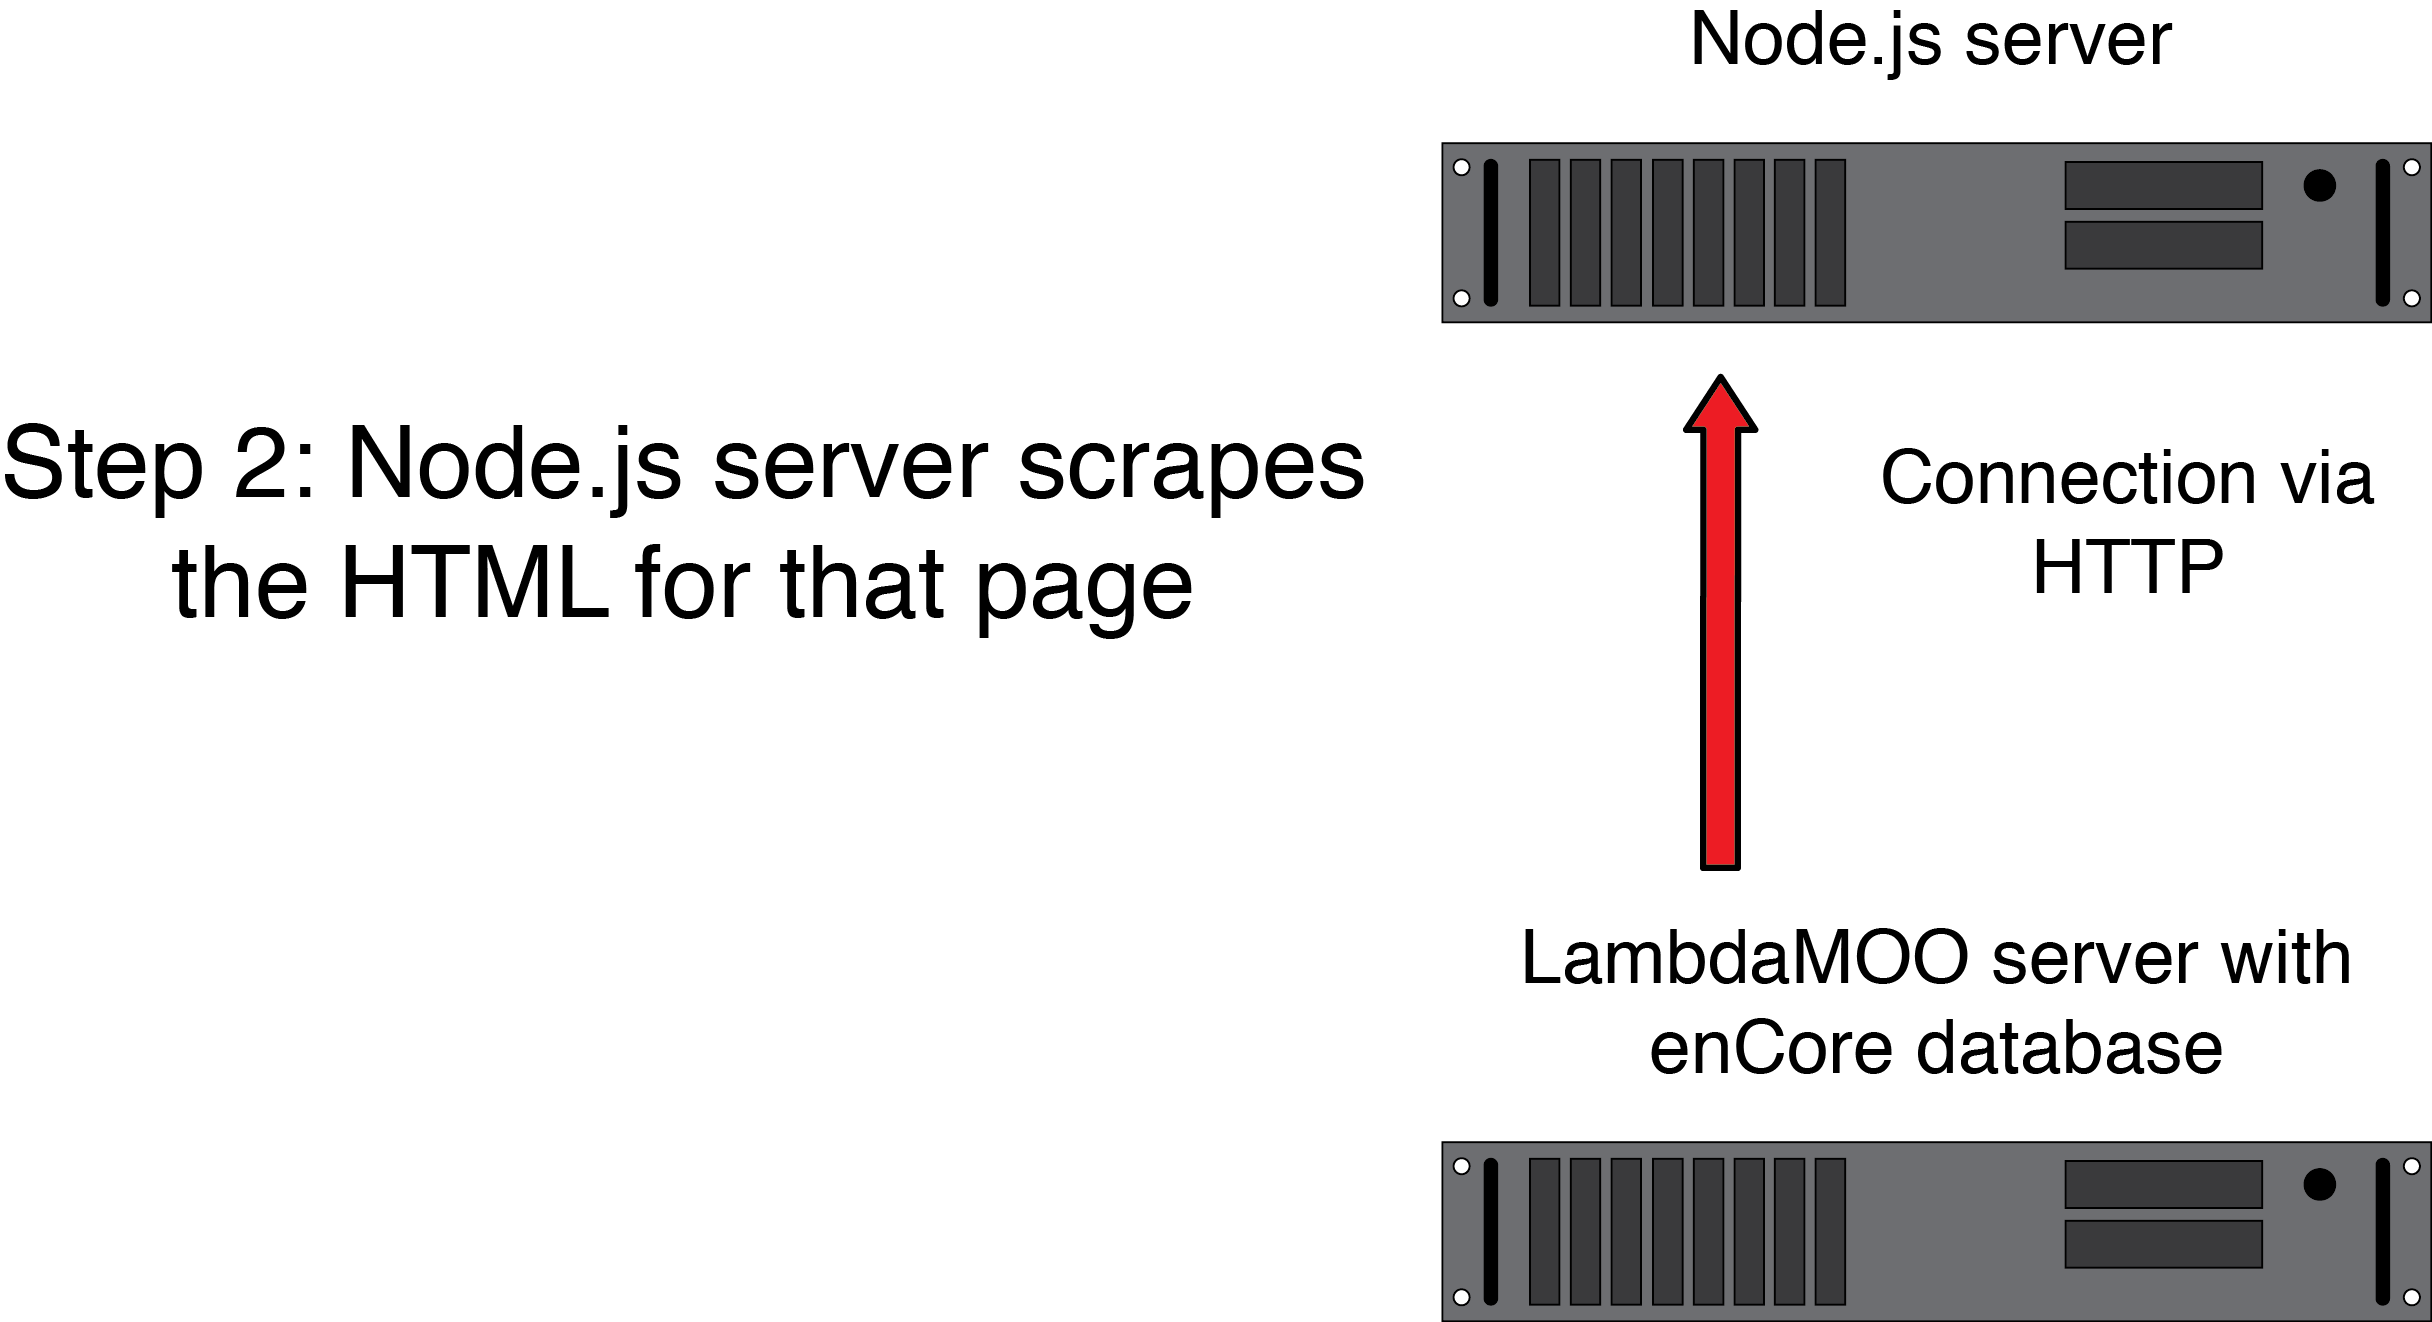
\includegraphics[width=\textwidth,height=\textheight,keepaspectratio]{NodeDiagram_2.png}
  \end{centering}
}

\frame{\frametitle{HTML sequence}
  \begin{centering}
  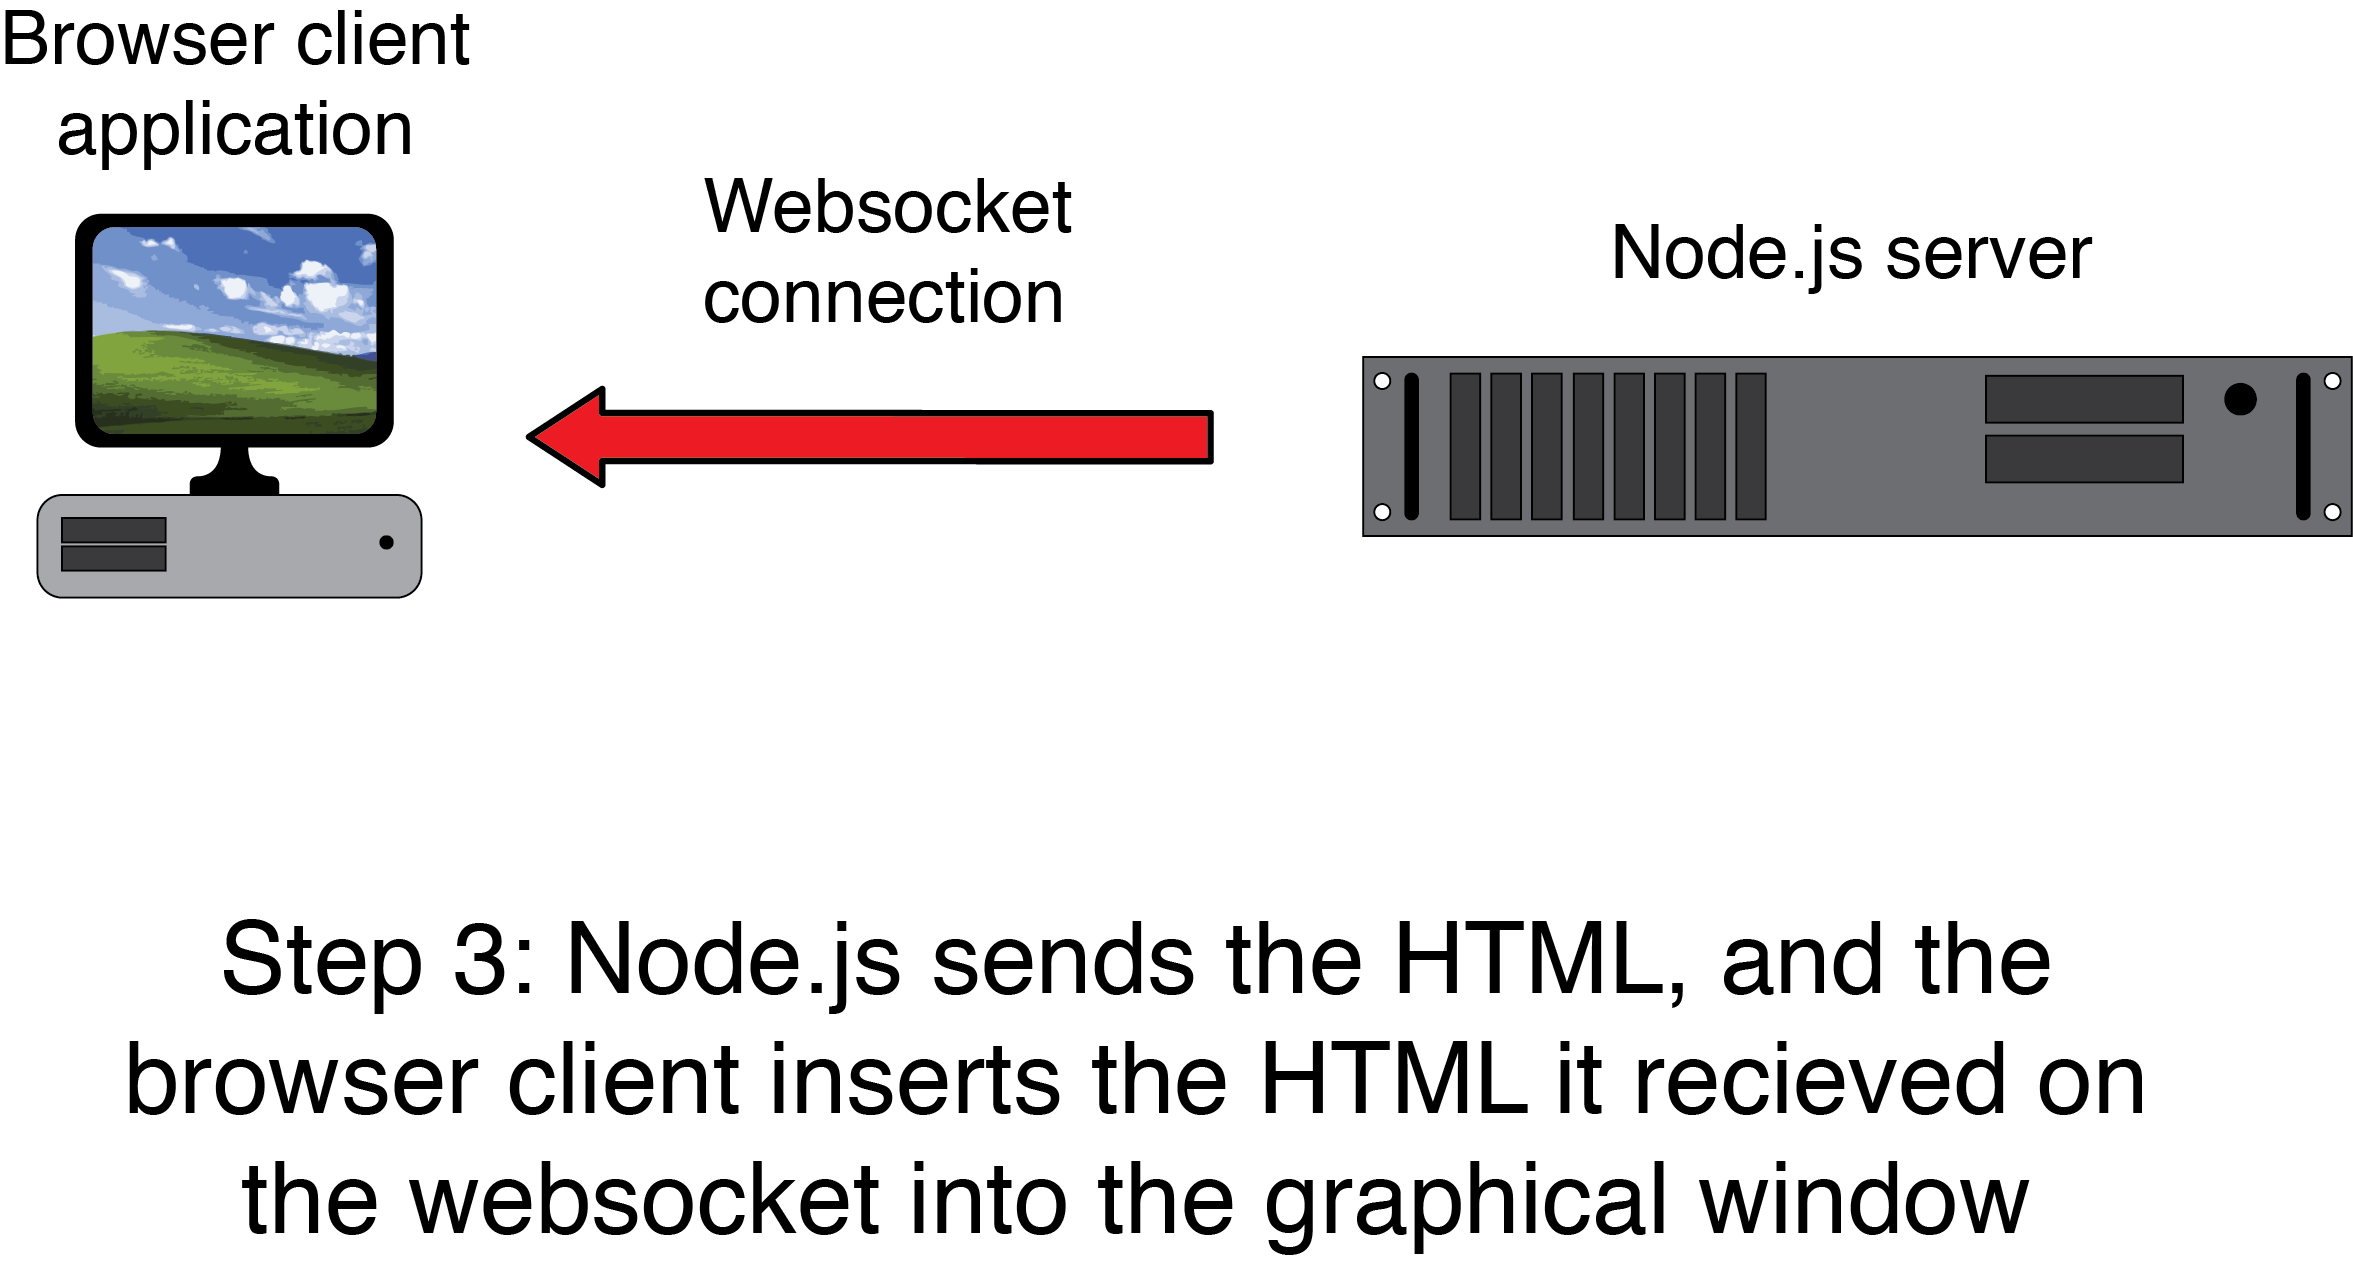
\includegraphics[width=\textwidth,height=\textheight,keepaspectratio]{NodeDiagram_3.png}
  \end{centering}
}

\frame{\frametitle{HTML sequence}
  \begin{centering}
  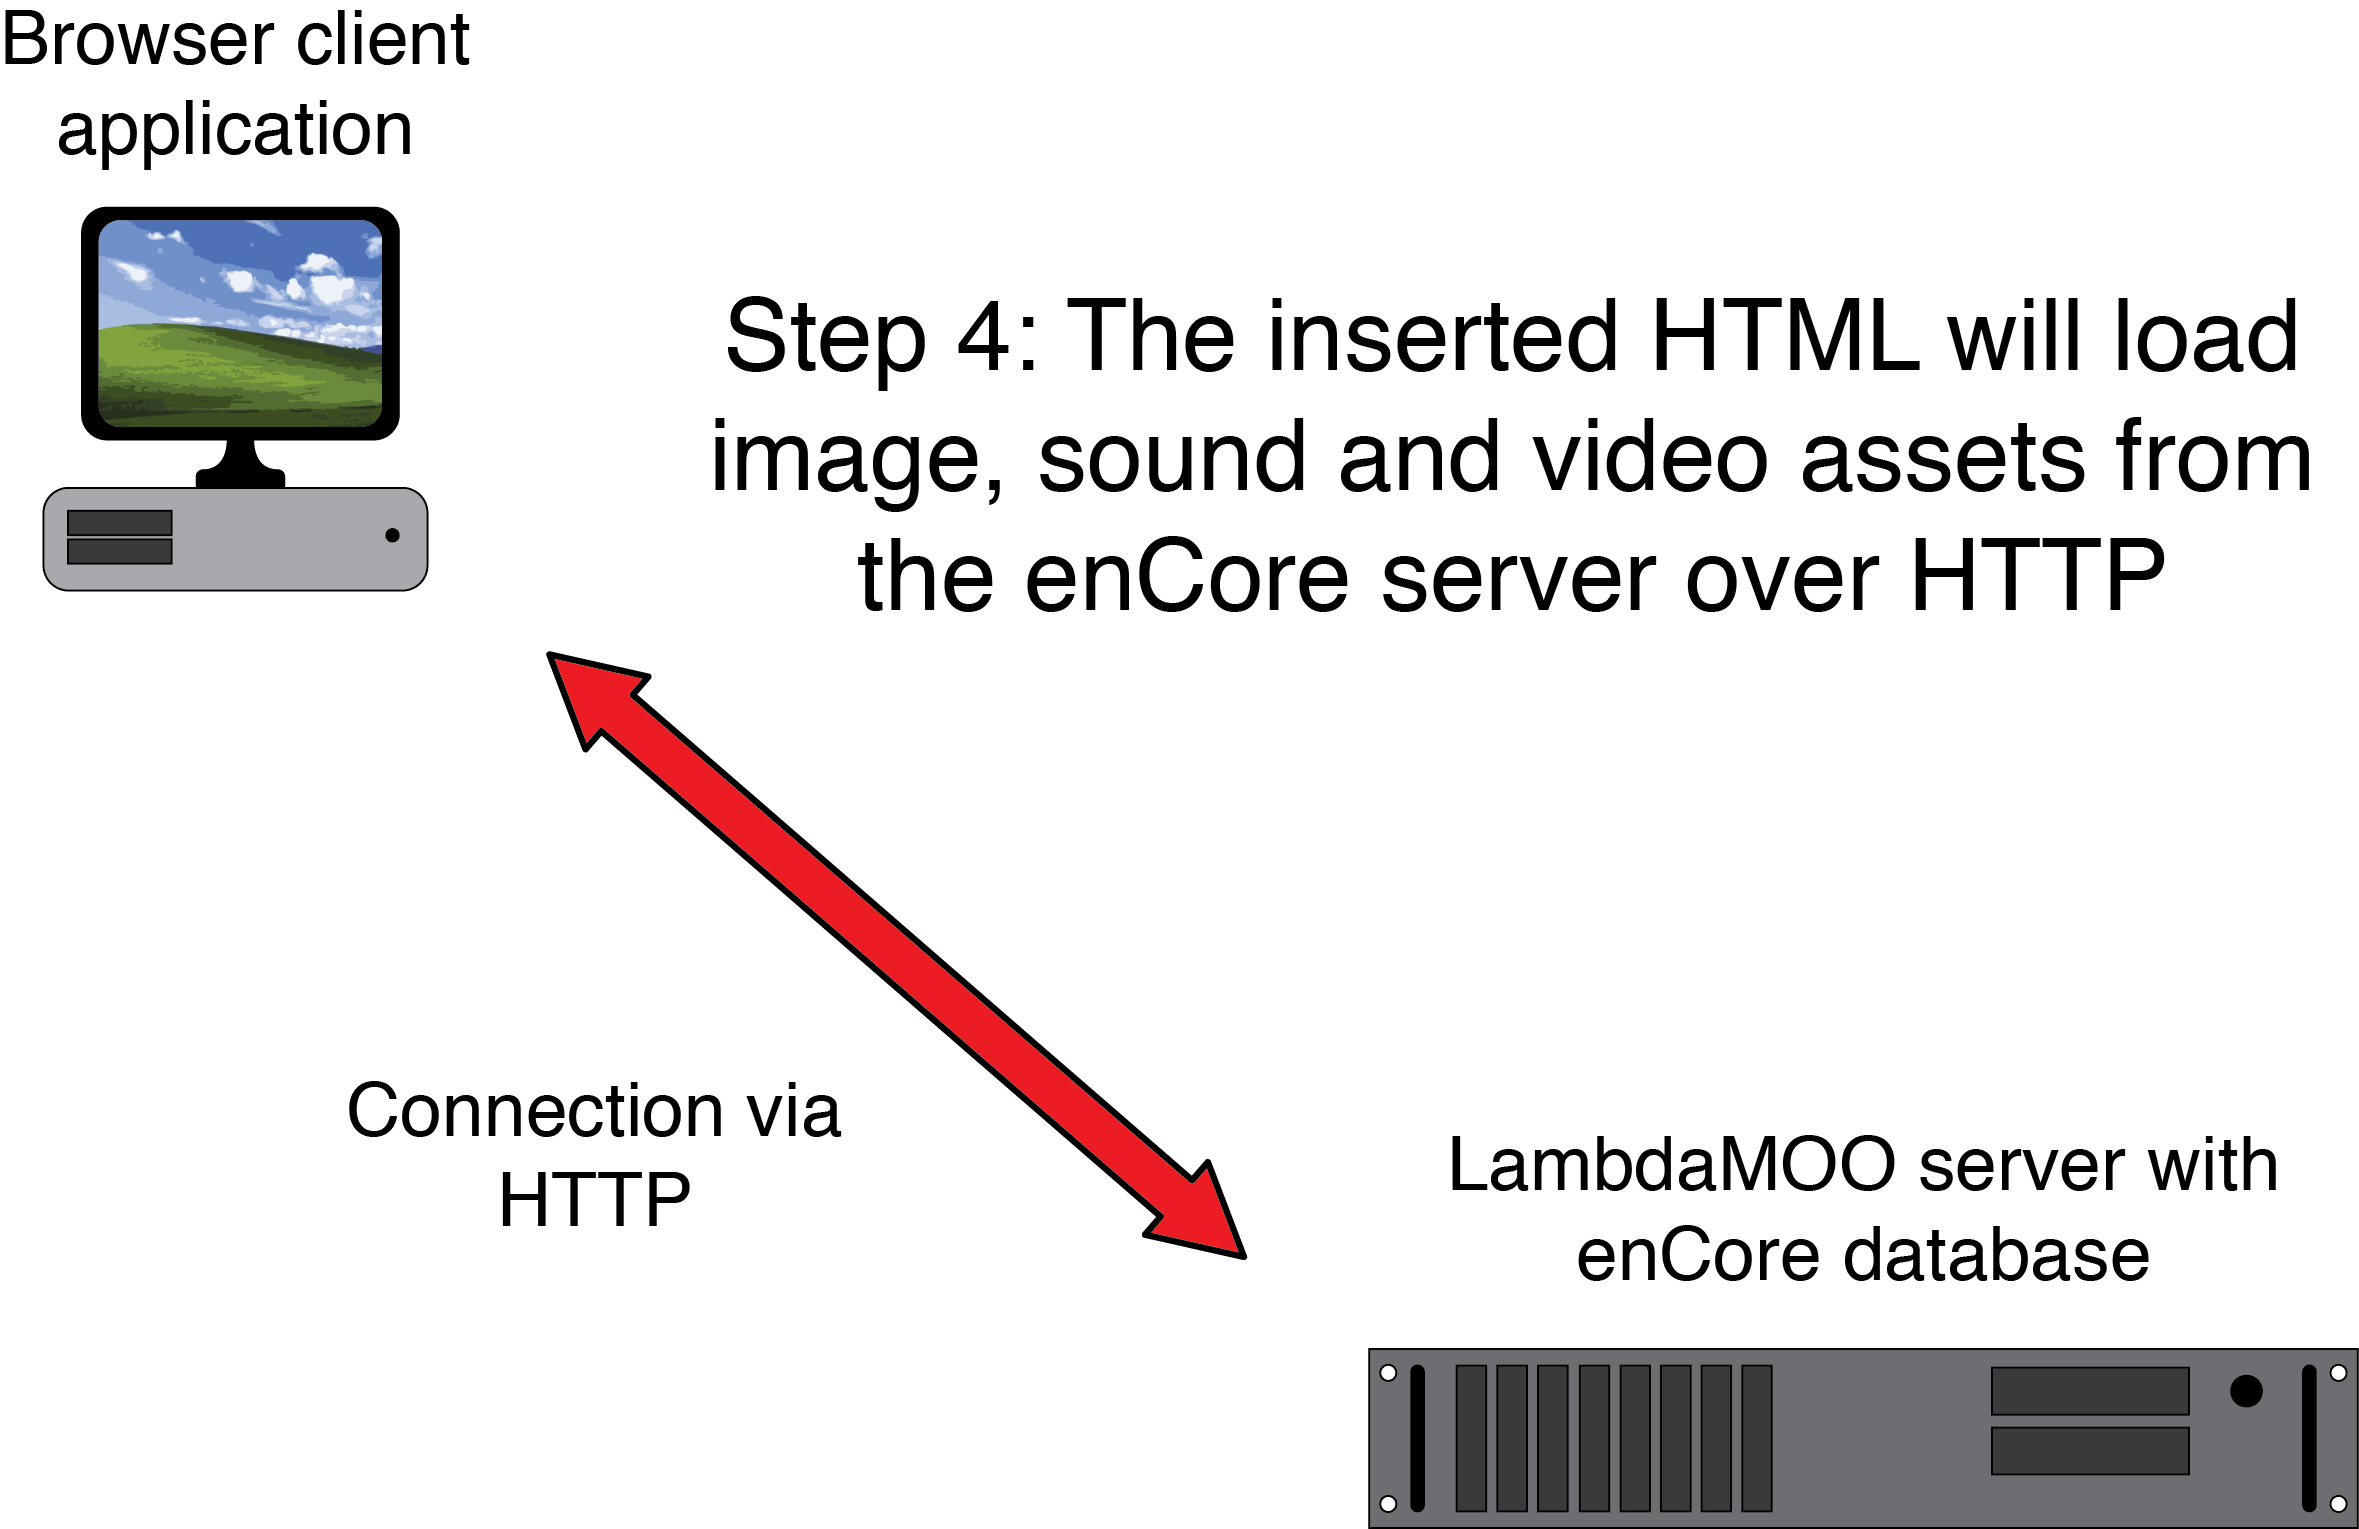
\includegraphics[width=\textwidth,height=\textheight,keepaspectratio]{NodeDiagram_4.png}
  \end{centering}
}


\frame{\frametitle{Future of the New Client}
\begin{itemize}
  \item Source code is hosted on Github
  \begin{itemize}
    \item Git is popular
    \item Github has a large community
  \end{itemize}
  \item Documentation will be created using Docco
  \begin{itemize}
  	\item HTML documentation is created
  	\item Comments displayed alongside code
  	\item Comments written in markdown
  \end{itemize}
  \item Grant may be obtained for updating Literary Worlds
\end{itemize}
}

\section{Testing}
\frame{\frametitle{Testing}
\begin{itemize}
    \item Unit Testing
    \begin{itemize}
      \item Each individual piece of code is tested
      \item This proves that the tested behaviour works
    \end{itemize}
    \item Functional Testing
      \begin{itemize}
        \item Test each world to compare functionality
      \end{itemize}
    \item Considerations
      \begin{itemize}
        \item Require.js is used to load client code
        \item Testing this is difficult
        \item Code structure provided by Backbone.js
      \end{itemize}
\end{itemize}
}

\frame{\frametitle{Testing - Jasmine}
\begin{centering}

\includegraphics[width=0.2\textwidth, height=\textheight,keepaspectratio,center]{jasmine.png}
\begin{itemize}
\item Jasmine - A testing framework for Javascript
\item Pros
\begin{itemize}
  \item Works with Node.js or browser code
  \item Large community
  \item Good documentation
  \item Readable, descriptive syntax
\end{itemize}
\item Cons
\begin{itemize}
  \item Loading code, dependencies and tests is difficult
\end{itemize}
\end{itemize}
\end{centering}
}

\section{Security}
\frame{\frametitle{Security}
  \begin{itemize}
    \item Security is not a main concern
    \item Telnet is vulnerable to eavesdropping
    \item Future project could implement SSL
  \end{itemize}
}

\frame{\frametitle{Summary}
  \begin{itemize}
  \item Literary Worlds uses a Java applet
  \item Used modern web technology to build new interface
  \item Did not change the users experience
  \item Removed the need for Java in browsers
  \end{itemize}
}

\frame{\frametitle{Questions}
\begin{centering}

\includegraphics[width=0.8\textwidth,height=0.8\textheight,keepaspectratio, center]{Help.png}
\end{centering}
}
\end{document}

